% ICLR 2027 submission, v5 (revision of v3, tag paper-d-iclr-v3). Numbers: papers/analysis/*.json (produced by committed scripts)
% and the registration ledgers. Run scripts/check_numbers.py before committing.

\documentclass{article}
\usepackage{iclr2027_conference,times}
%%%%% NEW MATH DEFINITIONS %%%%%

\usepackage{amsmath,amsfonts,bm}

% Mark sections of captions for referring to divisions of figures
\newcommand{\figleft}{{\em (Left)}}
\newcommand{\figcenter}{{\em (Center)}}
\newcommand{\figright}{{\em (Right)}}
\newcommand{\figtop}{{\em (Top)}}
\newcommand{\figbottom}{{\em (Bottom)}}
\newcommand{\captiona}{{\em (a)}}
\newcommand{\captionb}{{\em (b)}}
\newcommand{\captionc}{{\em (c)}}
\newcommand{\captiond}{{\em (d)}}

% Highlight a newly defined term
\newcommand{\newterm}[1]{{\bf #1}}


% Figure reference, lower-case.
\def\figref#1{figure~\ref{#1}}
% Figure reference, capital. For start of sentence
\def\Figref#1{Figure~\ref{#1}}
\def\twofigref#1#2{figures \ref{#1} and \ref{#2}}
\def\quadfigref#1#2#3#4{figures \ref{#1}, \ref{#2}, \ref{#3} and \ref{#4}}
% Section reference, lower-case.
\def\secref#1{section~\ref{#1}}
% Section reference, capital.
\def\Secref#1{Section~\ref{#1}}
% Reference to two sections.
\def\twosecrefs#1#2{sections \ref{#1} and \ref{#2}}
% Reference to three sections.
\def\secrefs#1#2#3{sections \ref{#1}, \ref{#2} and \ref{#3}}
% Reference to an equation, lower-case.
\def\eqref#1{equation~\ref{#1}}
% Reference to an equation, upper case
\def\Eqref#1{Equation~\ref{#1}}
% A raw reference to an equation---avoid using if possible
\def\plaineqref#1{\ref{#1}}
% Reference to a chapter, lower-case.
\def\chapref#1{chapter~\ref{#1}}
% Reference to an equation, upper case.
\def\Chapref#1{Chapter~\ref{#1}}
% Reference to a range of chapters
\def\rangechapref#1#2{chapters\ref{#1}--\ref{#2}}
% Reference to an algorithm, lower-case.
\def\algref#1{algorithm~\ref{#1}}
% Reference to an algorithm, upper case.
\def\Algref#1{Algorithm~\ref{#1}}
\def\twoalgref#1#2{algorithms \ref{#1} and \ref{#2}}
\def\Twoalgref#1#2{Algorithms \ref{#1} and \ref{#2}}
% Reference to a part, lower case
\def\partref#1{part~\ref{#1}}
% Reference to a part, upper case
\def\Partref#1{Part~\ref{#1}}
\def\twopartref#1#2{parts \ref{#1} and \ref{#2}}

\def\ceil#1{\lceil #1 \rceil}
\def\floor#1{\lfloor #1 \rfloor}
\def\1{\bm{1}}
\newcommand{\train}{\mathcal{D}}
\newcommand{\valid}{\mathcal{D_{\mathrm{valid}}}}
\newcommand{\test}{\mathcal{D_{\mathrm{test}}}}

\def\eps{{\epsilon}}


% Random variables
\def\reta{{\textnormal{$\eta$}}}
\def\ra{{\textnormal{a}}}
\def\rb{{\textnormal{b}}}
\def\rc{{\textnormal{c}}}
\def\rd{{\textnormal{d}}}
\def\re{{\textnormal{e}}}
\def\rf{{\textnormal{f}}}
\def\rg{{\textnormal{g}}}
\def\rh{{\textnormal{h}}}
\def\ri{{\textnormal{i}}}
\def\rj{{\textnormal{j}}}
\def\rk{{\textnormal{k}}}
\def\rl{{\textnormal{l}}}
% rm is already a command, just don't name any random variables m
\def\rn{{\textnormal{n}}}
\def\ro{{\textnormal{o}}}
\def\rp{{\textnormal{p}}}
\def\rq{{\textnormal{q}}}
\def\rr{{\textnormal{r}}}
\def\rs{{\textnormal{s}}}
\def\rt{{\textnormal{t}}}
\def\ru{{\textnormal{u}}}
\def\rv{{\textnormal{v}}}
\def\rw{{\textnormal{w}}}
\def\rx{{\textnormal{x}}}
\def\ry{{\textnormal{y}}}
\def\rz{{\textnormal{z}}}

% Random vectors
\def\rvepsilon{{\mathbf{\epsilon}}}
\def\rvtheta{{\mathbf{\theta}}}
\def\rva{{\mathbf{a}}}
\def\rvb{{\mathbf{b}}}
\def\rvc{{\mathbf{c}}}
\def\rvd{{\mathbf{d}}}
\def\rve{{\mathbf{e}}}
\def\rvf{{\mathbf{f}}}
\def\rvg{{\mathbf{g}}}
\def\rvh{{\mathbf{h}}}
\def\rvu{{\mathbf{i}}}
\def\rvj{{\mathbf{j}}}
\def\rvk{{\mathbf{k}}}
\def\rvl{{\mathbf{l}}}
\def\rvm{{\mathbf{m}}}
\def\rvn{{\mathbf{n}}}
\def\rvo{{\mathbf{o}}}
\def\rvp{{\mathbf{p}}}
\def\rvq{{\mathbf{q}}}
\def\rvr{{\mathbf{r}}}
\def\rvs{{\mathbf{s}}}
\def\rvt{{\mathbf{t}}}
\def\rvu{{\mathbf{u}}}
\def\rvv{{\mathbf{v}}}
\def\rvw{{\mathbf{w}}}
\def\rvx{{\mathbf{x}}}
\def\rvy{{\mathbf{y}}}
\def\rvz{{\mathbf{z}}}

% Elements of random vectors
\def\erva{{\textnormal{a}}}
\def\ervb{{\textnormal{b}}}
\def\ervc{{\textnormal{c}}}
\def\ervd{{\textnormal{d}}}
\def\erve{{\textnormal{e}}}
\def\ervf{{\textnormal{f}}}
\def\ervg{{\textnormal{g}}}
\def\ervh{{\textnormal{h}}}
\def\ervi{{\textnormal{i}}}
\def\ervj{{\textnormal{j}}}
\def\ervk{{\textnormal{k}}}
\def\ervl{{\textnormal{l}}}
\def\ervm{{\textnormal{m}}}
\def\ervn{{\textnormal{n}}}
\def\ervo{{\textnormal{o}}}
\def\ervp{{\textnormal{p}}}
\def\ervq{{\textnormal{q}}}
\def\ervr{{\textnormal{r}}}
\def\ervs{{\textnormal{s}}}
\def\ervt{{\textnormal{t}}}
\def\ervu{{\textnormal{u}}}
\def\ervv{{\textnormal{v}}}
\def\ervw{{\textnormal{w}}}
\def\ervx{{\textnormal{x}}}
\def\ervy{{\textnormal{y}}}
\def\ervz{{\textnormal{z}}}

% Random matrices
\def\rmA{{\mathbf{A}}}
\def\rmB{{\mathbf{B}}}
\def\rmC{{\mathbf{C}}}
\def\rmD{{\mathbf{D}}}
\def\rmE{{\mathbf{E}}}
\def\rmF{{\mathbf{F}}}
\def\rmG{{\mathbf{G}}}
\def\rmH{{\mathbf{H}}}
\def\rmI{{\mathbf{I}}}
\def\rmJ{{\mathbf{J}}}
\def\rmK{{\mathbf{K}}}
\def\rmL{{\mathbf{L}}}
\def\rmM{{\mathbf{M}}}
\def\rmN{{\mathbf{N}}}
\def\rmO{{\mathbf{O}}}
\def\rmP{{\mathbf{P}}}
\def\rmQ{{\mathbf{Q}}}
\def\rmR{{\mathbf{R}}}
\def\rmS{{\mathbf{S}}}
\def\rmT{{\mathbf{T}}}
\def\rmU{{\mathbf{U}}}
\def\rmV{{\mathbf{V}}}
\def\rmW{{\mathbf{W}}}
\def\rmX{{\mathbf{X}}}
\def\rmY{{\mathbf{Y}}}
\def\rmZ{{\mathbf{Z}}}

% Elements of random matrices
\def\ermA{{\textnormal{A}}}
\def\ermB{{\textnormal{B}}}
\def\ermC{{\textnormal{C}}}
\def\ermD{{\textnormal{D}}}
\def\ermE{{\textnormal{E}}}
\def\ermF{{\textnormal{F}}}
\def\ermG{{\textnormal{G}}}
\def\ermH{{\textnormal{H}}}
\def\ermI{{\textnormal{I}}}
\def\ermJ{{\textnormal{J}}}
\def\ermK{{\textnormal{K}}}
\def\ermL{{\textnormal{L}}}
\def\ermM{{\textnormal{M}}}
\def\ermN{{\textnormal{N}}}
\def\ermO{{\textnormal{O}}}
\def\ermP{{\textnormal{P}}}
\def\ermQ{{\textnormal{Q}}}
\def\ermR{{\textnormal{R}}}
\def\ermS{{\textnormal{S}}}
\def\ermT{{\textnormal{T}}}
\def\ermU{{\textnormal{U}}}
\def\ermV{{\textnormal{V}}}
\def\ermW{{\textnormal{W}}}
\def\ermX{{\textnormal{X}}}
\def\ermY{{\textnormal{Y}}}
\def\ermZ{{\textnormal{Z}}}

% Vectors
\def\vzero{{\bm{0}}}
\def\vone{{\bm{1}}}
\def\vmu{{\bm{\mu}}}
\def\vtheta{{\bm{\theta}}}
\def\va{{\bm{a}}}
\def\vb{{\bm{b}}}
\def\vc{{\bm{c}}}
\def\vd{{\bm{d}}}
\def\ve{{\bm{e}}}
\def\vf{{\bm{f}}}
\def\vg{{\bm{g}}}
\def\vh{{\bm{h}}}
\def\vi{{\bm{i}}}
\def\vj{{\bm{j}}}
\def\vk{{\bm{k}}}
\def\vl{{\bm{l}}}
\def\vm{{\bm{m}}}
\def\vn{{\bm{n}}}
\def\vo{{\bm{o}}}
\def\vp{{\bm{p}}}
\def\vq{{\bm{q}}}
\def\vr{{\bm{r}}}
\def\vs{{\bm{s}}}
\def\vt{{\bm{t}}}
\def\vu{{\bm{u}}}
\def\vv{{\bm{v}}}
\def\vw{{\bm{w}}}
\def\vx{{\bm{x}}}
\def\vy{{\bm{y}}}
\def\vz{{\bm{z}}}

% Elements of vectors
\def\evalpha{{\alpha}}
\def\evbeta{{\beta}}
\def\evepsilon{{\epsilon}}
\def\evlambda{{\lambda}}
\def\evomega{{\omega}}
\def\evmu{{\mu}}
\def\evpsi{{\psi}}
\def\evsigma{{\sigma}}
\def\evtheta{{\theta}}
\def\eva{{a}}
\def\evb{{b}}
\def\evc{{c}}
\def\evd{{d}}
\def\eve{{e}}
\def\evf{{f}}
\def\evg{{g}}
\def\evh{{h}}
\def\evi{{i}}
\def\evj{{j}}
\def\evk{{k}}
\def\evl{{l}}
\def\evm{{m}}
\def\evn{{n}}
\def\evo{{o}}
\def\evp{{p}}
\def\evq{{q}}
\def\evr{{r}}
\def\evs{{s}}
\def\evt{{t}}
\def\evu{{u}}
\def\evv{{v}}
\def\evw{{w}}
\def\evx{{x}}
\def\evy{{y}}
\def\evz{{z}}

% Matrix
\def\mA{{\bm{A}}}
\def\mB{{\bm{B}}}
\def\mC{{\bm{C}}}
\def\mD{{\bm{D}}}
\def\mE{{\bm{E}}}
\def\mF{{\bm{F}}}
\def\mG{{\bm{G}}}
\def\mH{{\bm{H}}}
\def\mI{{\bm{I}}}
\def\mJ{{\bm{J}}}
\def\mK{{\bm{K}}}
\def\mL{{\bm{L}}}
\def\mM{{\bm{M}}}
\def\mN{{\bm{N}}}
\def\mO{{\bm{O}}}
\def\mP{{\bm{P}}}
\def\mQ{{\bm{Q}}}
\def\mR{{\bm{R}}}
\def\mS{{\bm{S}}}
\def\mT{{\bm{T}}}
\def\mU{{\bm{U}}}
\def\mV{{\bm{V}}}
\def\mW{{\bm{W}}}
\def\mX{{\bm{X}}}
\def\mY{{\bm{Y}}}
\def\mZ{{\bm{Z}}}
\def\mBeta{{\bm{\beta}}}
\def\mPhi{{\bm{\Phi}}}
\def\mLambda{{\bm{\Lambda}}}
\def\mSigma{{\bm{\Sigma}}}

% Tensor
\DeclareMathAlphabet{\mathsfit}{\encodingdefault}{\sfdefault}{m}{sl}
\SetMathAlphabet{\mathsfit}{bold}{\encodingdefault}{\sfdefault}{bx}{n}
\newcommand{\tens}[1]{\bm{\mathsfit{#1}}}
\def\tA{{\tens{A}}}
\def\tB{{\tens{B}}}
\def\tC{{\tens{C}}}
\def\tD{{\tens{D}}}
\def\tE{{\tens{E}}}
\def\tF{{\tens{F}}}
\def\tG{{\tens{G}}}
\def\tH{{\tens{H}}}
\def\tI{{\tens{I}}}
\def\tJ{{\tens{J}}}
\def\tK{{\tens{K}}}
\def\tL{{\tens{L}}}
\def\tM{{\tens{M}}}
\def\tN{{\tens{N}}}
\def\tO{{\tens{O}}}
\def\tP{{\tens{P}}}
\def\tQ{{\tens{Q}}}
\def\tR{{\tens{R}}}
\def\tS{{\tens{S}}}
\def\tT{{\tens{T}}}
\def\tU{{\tens{U}}}
\def\tV{{\tens{V}}}
\def\tW{{\tens{W}}}
\def\tX{{\tens{X}}}
\def\tY{{\tens{Y}}}
\def\tZ{{\tens{Z}}}


% Graph
\def\gA{{\mathcal{A}}}
\def\gB{{\mathcal{B}}}
\def\gC{{\mathcal{C}}}
\def\gD{{\mathcal{D}}}
\def\gE{{\mathcal{E}}}
\def\gF{{\mathcal{F}}}
\def\gG{{\mathcal{G}}}
\def\gH{{\mathcal{H}}}
\def\gI{{\mathcal{I}}}
\def\gJ{{\mathcal{J}}}
\def\gK{{\mathcal{K}}}
\def\gL{{\mathcal{L}}}
\def\gM{{\mathcal{M}}}
\def\gN{{\mathcal{N}}}
\def\gO{{\mathcal{O}}}
\def\gP{{\mathcal{P}}}
\def\gQ{{\mathcal{Q}}}
\def\gR{{\mathcal{R}}}
\def\gS{{\mathcal{S}}}
\def\gT{{\mathcal{T}}}
\def\gU{{\mathcal{U}}}
\def\gV{{\mathcal{V}}}
\def\gW{{\mathcal{W}}}
\def\gX{{\mathcal{X}}}
\def\gY{{\mathcal{Y}}}
\def\gZ{{\mathcal{Z}}}

% Sets
\def\sA{{\mathbb{A}}}
\def\sB{{\mathbb{B}}}
\def\sC{{\mathbb{C}}}
\def\sD{{\mathbb{D}}}
% Don't use a set called E, because this would be the same as our symbol
% for expectation.
\def\sF{{\mathbb{F}}}
\def\sG{{\mathbb{G}}}
\def\sH{{\mathbb{H}}}
\def\sI{{\mathbb{I}}}
\def\sJ{{\mathbb{J}}}
\def\sK{{\mathbb{K}}}
\def\sL{{\mathbb{L}}}
\def\sM{{\mathbb{M}}}
\def\sN{{\mathbb{N}}}
\def\sO{{\mathbb{O}}}
\def\sP{{\mathbb{P}}}
\def\sQ{{\mathbb{Q}}}
\def\sR{{\mathbb{R}}}
\def\sS{{\mathbb{S}}}
\def\sT{{\mathbb{T}}}
\def\sU{{\mathbb{U}}}
\def\sV{{\mathbb{V}}}
\def\sW{{\mathbb{W}}}
\def\sX{{\mathbb{X}}}
\def\sY{{\mathbb{Y}}}
\def\sZ{{\mathbb{Z}}}

% Entries of a matrix
\def\emLambda{{\Lambda}}
\def\emA{{A}}
\def\emB{{B}}
\def\emC{{C}}
\def\emD{{D}}
\def\emE{{E}}
\def\emF{{F}}
\def\emG{{G}}
\def\emH{{H}}
\def\emI{{I}}
\def\emJ{{J}}
\def\emK{{K}}
\def\emL{{L}}
\def\emM{{M}}
\def\emN{{N}}
\def\emO{{O}}
\def\emP{{P}}
\def\emQ{{Q}}
\def\emR{{R}}
\def\emS{{S}}
\def\emT{{T}}
\def\emU{{U}}
\def\emV{{V}}
\def\emW{{W}}
\def\emX{{X}}
\def\emY{{Y}}
\def\emZ{{Z}}
\def\emSigma{{\Sigma}}

% entries of a tensor
% Same font as tensor, without \bm wrapper
\newcommand{\etens}[1]{\mathsfit{#1}}
\def\etLambda{{\etens{\Lambda}}}
\def\etA{{\etens{A}}}
\def\etB{{\etens{B}}}
\def\etC{{\etens{C}}}
\def\etD{{\etens{D}}}
\def\etE{{\etens{E}}}
\def\etF{{\etens{F}}}
\def\etG{{\etens{G}}}
\def\etH{{\etens{H}}}
\def\etI{{\etens{I}}}
\def\etJ{{\etens{J}}}
\def\etK{{\etens{K}}}
\def\etL{{\etens{L}}}
\def\etM{{\etens{M}}}
\def\etN{{\etens{N}}}
\def\etO{{\etens{O}}}
\def\etP{{\etens{P}}}
\def\etQ{{\etens{Q}}}
\def\etR{{\etens{R}}}
\def\etS{{\etens{S}}}
\def\etT{{\etens{T}}}
\def\etU{{\etens{U}}}
\def\etV{{\etens{V}}}
\def\etW{{\etens{W}}}
\def\etX{{\etens{X}}}
\def\etY{{\etens{Y}}}
\def\etZ{{\etens{Z}}}

% The true underlying data generating distribution
\newcommand{\pdata}{p_{\rm{data}}}
% The empirical distribution defined by the training set
\newcommand{\ptrain}{\hat{p}_{\rm{data}}}
\newcommand{\Ptrain}{\hat{P}_{\rm{data}}}
% The model distribution
\newcommand{\pmodel}{p_{\rm{model}}}
\newcommand{\Pmodel}{P_{\rm{model}}}
\newcommand{\ptildemodel}{\tilde{p}_{\rm{model}}}
% Stochastic autoencoder distributions
\newcommand{\pencode}{p_{\rm{encoder}}}
\newcommand{\pdecode}{p_{\rm{decoder}}}
\newcommand{\precons}{p_{\rm{reconstruct}}}

\newcommand{\laplace}{\mathrm{Laplace}} % Laplace distribution

\newcommand{\E}{\mathbb{E}}
\newcommand{\Ls}{\mathcal{L}}
\newcommand{\R}{\mathbb{R}}
\newcommand{\emp}{\tilde{p}}
\newcommand{\lr}{\alpha}
\newcommand{\reg}{\lambda}
\newcommand{\rect}{\mathrm{rectifier}}
\newcommand{\softmax}{\mathrm{softmax}}
\newcommand{\sigmoid}{\sigma}
\newcommand{\softplus}{\zeta}
\newcommand{\KL}{D_{\mathrm{KL}}}
\newcommand{\Var}{\mathrm{Var}}
\newcommand{\standarderror}{\mathrm{SE}}
\newcommand{\Cov}{\mathrm{Cov}}
% Wolfram Mathworld says $L^2$ is for function spaces and $\ell^2$ is for vectors
% But then they seem to use $L^2$ for vectors throughout the site, and so does
% wikipedia.
\newcommand{\normlzero}{L^0}
\newcommand{\normlone}{L^1}
\newcommand{\normltwo}{L^2}
\newcommand{\normlp}{L^p}
\newcommand{\normmax}{L^\infty}

\newcommand{\parents}{Pa} % See usage in notation.tex. Chosen to match Daphne's book.

\DeclareMathOperator*{\argmax}{arg\,max}
\DeclareMathOperator*{\argmin}{arg\,min}

\DeclareMathOperator{\sign}{sign}
\DeclareMathOperator{\Tr}{Tr}
\let\ab\allowbreak


\usepackage{amsmath,amssymb}
\usepackage{graphicx}
\usepackage{booktabs}
\usepackage{array}
\usepackage{xcolor}
\usepackage[colorlinks=true,linkcolor={blue!50!black},citecolor={blue!50!black},urlcolor={blue!50!black}]{hyperref}
\usepackage{url}
\usepackage[capitalise,noabbrev]{cleveref}
\usepackage{caption}
\captionsetup{font=small,labelfont=bf}
\captionsetup[table]{skip=4pt}
\usepackage{enumitem}
\usepackage{longtable}
\usepackage{adjustbox}
\usepackage{xspace}
\usepackage{placeins}
\usepackage{tikz}
\usetikzlibrary{arrows.meta,positioning,calc}

\newcommand{\sd}{\textsc{sd}\xspace}
\newcommand{\ci}[2]{{\scriptsize$[#1,#2]$}}
\newcolumntype{L}[1]{>{\raggedright\arraybackslash}p{#1}}
% Registration status. Main text: unmarked = pre-specified (OSF or timestamped commit); dagger = post hoc;
% double dagger = pre-specified re-analysis of an effect whose direction was known. The appendix keeps the full labels.
\newcommand{\osf}{\textsuperscript{\textsc{osf}}}
\newcommand{\pre}{\textsuperscript{\textsc{pre}}}
\newcommand{\reana}{\textsuperscript{$\ddagger$}}
\newcommand{\ph}{\textsuperscript{$\dagger$}}
\newcommand{\pending}[1]{\textcolor{red}{#1}}

\title{Reference Anchoring Biases LLM Judges\\Toward the Answer They Are Shown\\When Several Are Correct}

\author{Anonymous authors\\Paper under double-blind review}

\begin{document}
\maketitle
\raggedbottom

\begin{abstract}
LLM judges often grade against a reference answer: 35 of the 43 benchmarks, libraries, platforms, and RL reward pipelines we surveyed do, including those shipped with SimpleQA, BrowseComp, and Humanity's Last Exam.
The premise is that the reference acts as an answer key: a correct response should score the same whichever correct answer is shown.
With one correct answer the premise holds and the reference helps, raising best-of-64 accuracy sharply (\cref{sec:p2}); with several, it fails.
We test it with more than a dozen judges, open models up to 14B and frontier API judges, on constructed tasks, MACE, and MATH-500, with a full preregistration ledger.
(1) Swapping the reference between two correct answers moves the score of identical text by about 3 to 5 points out of 10.
(2) Correct answers that differ from the reference are graded worse against wrong answers, for the four open judges under every labeling we tried.
(3) Judges take back credit: of 843 differing correct answers two frontier judges accepted blind, 117 drop to 3 or below once the reference is shown, against 2 on a repeated blind call.
Those benchmarks rarely contain such questions. Run verbatim on 149 factual questions that do, with the reference drawn at random, their graders credit 0\% to 53\% of correct answers that differ from it and score four models 30 to 67 points below answer-list accuracy; choosing the reference instead leaves two of those graders 9 to 56 points short.
Much of this comes from the instruction to match: asked instead whether the answer is correct, judges shrink the gap on questions they can answer.
Given the full answer list, the graders come within a point of answer-list accuracy, partly by construction, since those lists define correctness, though one open verifier stays far short.
Where several answers are correct, a low score from a reference-guided judge does not reliably mean the answer is wrong.
\end{abstract}

\begin{figure}[!b]
\centering
\resizebox{0.64\textwidth}{!}{% Figure 1: the finding. (a) a real replication-pool task (repl/digitsum-116; candidate sample 16 from Llama-3.1-8B,
% abridged verbatim); (b) the same text scored blind and with each correct answer as the reference (Qwen2.5-7B, exact
% scorer: runs/r4/scores repl noref/ref and replrot ref). v3: the pool-level swap plot (v2 panel c) moved to the appendix,
% and the pool-level false-rejection note moved to Section 5.
% Sans-serif throughout so the text matches the matplotlib panel.
\definecolor{refblue}{HTML}{4269D0}
\definecolor{blindorange}{HTML}{C5541A}
\definecolor{penalred}{HTML}{A51C30}
\begin{tikzpicture}[
  font=\sffamily\footnotesize,
  >={Stealth[length=4pt]},
  panel/.style={font=\sffamily\footnotesize\bfseries, anchor=west},
  box/.style={draw=black!45, rounded corners=2pt, fill=black!3, align=left, inner sep=4pt},
  refbox/.style={draw=refblue, rounded corners=2pt, fill=refblue!8, align=center, inner sep=3pt, minimum width=2.05cm},
  blindbox/.style={draw=blindorange, rounded corners=2pt, fill=blindorange!8, align=center, inner sep=3pt, minimum width=2.05cm},
  judge/.style={draw=black!70, rounded corners=3pt, fill=black!8, align=center, inner sep=3pt, minimum width=1.0cm, minimum height=0.55cm},
  score/.style={align=center, inner sep=2pt, font=\sffamily\small},
]
% ---------------- (a) the task
\node[panel] at (0, 2.6) {a\;\;The task};
\node[box, text width=3.45cm, anchor=north west] (q) at (0, 2.3) {%
  \textbf{Question.} Give one 2-digit number that is divisible by 5 and whose digits sum to 8.\\[3pt]
  \textbf{Correct answers.} 35 and 80.\\[3pt]
  \textbf{Candidate} (fixed text, abridged):\\
  \textsl{``\ldots\ the ones digit is 0. In this case, the tens digit must be 8 \ldots\ The answer is 80.''}};

% ---------------- (b) one candidate, three prompts
\node[panel] at (4.0, 2.6) {b\;\;Same text, three prompts};
\node[blindbox] (c0) at (5.1, 1.95) {no reference};
\node[refbox] (c1) at (5.1, 1.15) {reference: \textbf{35}};
\node[refbox] (c2) at (5.1, 0.35) {reference: \textbf{80}};
\node[judge] (j0) at (6.85, 1.95) {judge};
\node[judge] (j1) at (6.85, 1.15) {judge};
\node[judge] (j2) at (6.85, 0.35) {judge};
\foreach \i in {0,1,2} {\draw[->, black!60] (c\i) -- (j\i);}
\node[score, text=blindorange] (s0) at (7.85, 1.95) {10.0};
\node[score, text=penalred] (s1) at (7.85, 1.15) {\textbf{2.9}};
\node[score, text=refblue] (s2) at (7.85, 0.35) {\textbf{9.3}};
\foreach \i in {0,1,2} {\draw[->, black!60] (j\i) -- (s\i);}
\node[font=\sffamily\footnotesize, text=black!75, align=left, anchor=north west, text width=4.1cm, inner sep=0pt] at (4.0, -0.15) {Judge: Qwen2.5-7B, score out of 10.};

\end{tikzpicture}
}
\caption{\textbf{A judge's score follows the correct answer it is shown.}
\textbf{(a)}~A constructed task with two correct answers and one of its candidate replies (abridged; selection rule and full reply in \cref{app:setup}).
\textbf{(b)}~Qwen2.5-7B scores the same text without a reference and with each correct answer as the reference. The example was selected for a large, clean swap; over the whole pool the swap is about 5 points for this judge (\cref{sec:p1}).}
\label{fig:concept}
\end{figure}

\section{Introduction}
\label{sec:intro}

Ask for a two-digit number that is divisible by 5 and whose digits sum to 8.
Both 35 and 80 are correct.
Qwen2.5-7B, shown a candidate that reasons its way to 80, scores it 10.0 out of 10 with no reference, 2.9 when the reference answer is 35, and 9.3 when the reference is 80 (\cref{fig:concept}b).
The text never changed; only the correct answer the judge was shown did.
This example swaps more than most, but over 120 such tasks the same judge moves correct text by about 5 points in either direction (\cref{sec:p1}).

Reference-guided judging is how many benchmarks are scored.
The judge used by BrowseComp and Humanity's Last Exam (HLE), for example, is told ``do not argue for any answer different than [correct\_answer]''~\citep{wei2025browsecomp,phan2025hle}.
Of 43 benchmarks, evaluation libraries, platforms, and RL reward pipelines we checked, 35 grade with a single reference or a closed list, and none of the judge prompts we could read tells the judge to credit a correct answer outside it (\cref{app:survey}).\ph{}
The same judges also pick the best of several sampled answers and serve as reward signals, which optimization exploits~\citep{gao2022scaling}.
The problem is not confined to math: factual answers, agent outputs, informal proofs, and RL rewards have no formal checker, which is why LLM judges grade them. We use arithmetic as a controlled testbed, because a checker lists every correct answer, and factual questions because benchmark graders operate there.

\paragraph{What the reference could be doing.}
Either the judge checks a candidate against every correct answer, so the reference acts as an answer key, or it rewards the one correct answer it was shown.
P1 and P2 rule out the first; P3 checks that the second is not merely an inability to recognize the other correct answers:
\begin{itemize}[leftmargin=1.5em,itemsep=0pt,topsep=0pt]
\item[\textbf{P1}] \textbf{The score follows the reference.} Swapping which correct answer is the reference moves the score of unchanged text (\cref{sec:p1}).
\item[\textbf{P2}] \textbf{Correct answers that differ from the reference are graded worse.} With several correct answers they lose ground against wrong answers; with one, matching the reference and being correct coincide, so the reference should help (\cref{sec:p2}).
\item[\textbf{P3}] \textbf{The effect persists after blind acceptance.} It remains for correct answers the judge already accepts without a reference, so it is not only that the judge cannot verify them (\cref{sec:p3}).
\end{itemize}

\paragraph{What we find.}
All three predictions hold (\cref{tab:summary}), and the effect matters in practice.
Run as their authors configure them, the graders of SimpleQA, BrowseComp, and HLE score four models 30 to 67 points below what the full answer lists say their answers are worth (\cref{sec:cost}).
Much of that gap comes from the instruction to match: asking whether the answer is correct shrinks it where the judge can answer the question, although on harder questions one of our two judges then accepted wrong answers.
Giving the grader the full answer list nearly closes it, though one open verifier does not follow the list (\cref{sec:fix}).
Prior work comes close without isolating this failure.
\citet{fixation2025} name ``solution fixation'' but measure it with flawed solutions rewritten in the reference's style, and \citet{judgingref2026} and \citet{krumdick2025nofreelabels} replace the reference with a wrong one.
Question-answering evaluation has long under-credited correct answers missing from a gold list~\citep{min2020ambigqa,kamalloo2023evaluating}; here the list is complete and the judge still favors the answer it was shown.

\begin{table}[t]
\centering
\small
\caption{\textbf{What each prediction tests and what we observed.} Each row's numbers, intervals, and failed registered predictions are in the cited section and the ledger (\cref{app:ledger}).}
\label{tab:summary}
\setlength{\tabcolsep}{4pt}
\renewcommand{\arraystretch}{1.0}
\begin{tabular}{L{2.9cm}L{2.0cm}L{5.0cm}L{2.7cm}}
\toprule
Question & Rules out & Key evidence & Verdict \\
\midrule
\textbf{P1} Does the score follow the reference? & Answer key & Identical text moves 3--5 points when the reference moves to another correct answer (\cref{sec:p1}) & Holds; near zero on arithmetic for a thinking judge \\
\textbf{P2} Are differing correct answers graded worse? & Answer key & Their grading against wrong answers drops under every answer labeling; with one correct answer the reference helps (\cref{sec:p2}) & Holds. Small for API judges on arithmetic; interval includes zero for GPT-4.1 (factual) and Opus~5 (replication pool) \\
\textbf{P3} Does it persist after blind acceptance? & Inability to verify, on its own & Answers accepted blind are rejected once another correct answer is the reference; a repeated blind call almost never does this (\cref{sec:p3}) & Holds for every judge with an acceptance test \\
\emph{Consequence} & --- & Shipped benchmark graders and RL verifiers under-credit such answers heavily (\cref{sec:cost}) & Large on questions with several answers; those are rare on the shipped benchmarks \\
\emph{Fix} & --- & A full answer list closes the gap for the benchmark graders; correctness prompts shrink it but can admit wrong answers on hard questions (\cref{sec:fix}) & The list works, except for one 1.5B verifier \\
\bottomrule
\end{tabular}
\end{table}

\section{Setup}
\label{sec:setup}

\paragraph{Tasks.}
Our own tasks come from five constraint families (remainder systems, subset sums, Goldbach pairs, divisor counts, digit sums); each stores its full set of correct answers and one member, drawn at random, as the reference.
The \emph{replication pool} (120 tasks) was built to replicate an exploratory observation on \textsc{RewardBench-2} Ties~\citep{malik2025rewardbench2}; the \emph{$k$-pool} has 75 tasks with exactly $k \in \{1,2,4,8,16\}$ correct answers.
\textsc{MACE}~\citep{mace2026} contributes factual questions with 1, 2, 4, or 6 correct answers from its River and Language domains, where a model's valid answer is missing from the list 2.3\% and 8.1\% of the time.
The reference is drawn at random from each list, and an answer matches it by normalized string containment (\cref{app:mace}).
MATH-500~\citep{hendrycks2021math} supplies unique answers.

\paragraph{Candidates, judges, and prompts.}
\begin{itemize}[leftmargin=1.2em,itemsep=0pt,topsep=0pt]
\item \textbf{Candidates.} Llama-3.1-8B-Instruct~\citep{grattafiori2024llama3} writes 64 samples per task at temperature 1 (Qwen2.5-7B for MATH-500).
\item \textbf{Conditions.} Each sample is judged \emph{blind}, from the question and the candidate, and \emph{referenced}, with the reference under the heading ``Reference answer (trusted)''.
\item \textbf{Open judges.} Qwen2.5-7B and Qwen2.5-14B~\citep{yang2024qwen25}, phi-4~\citep{abdin2024phi4}, and gemma-2-9b~\citep{riviere2024gemma2} output only a score, of which we use the expected value over the score tokens; a fifth, Mistral-7B, fails a score-resolution screen (\cref{app:setup,app:mitigation}).
\item \textbf{API judges.} Claude Sonnet~5 and Opus~5, with thinking disabled, score 16-candidate subsamples of each pool that always include a matching correct answer, a differing correct answer, and a wrong answer. GPT-4.1's scores tie too often to rank candidates, so we use it for grading only.
\item \textbf{Benchmark graders} (\cref{sec:cost}). The SimpleQA and BrowseComp/HLE graders run with GPT-4.1, o3-mini, and Sonnet~5; our rubric also runs with Opus~5 and Haiku~4.5; and two open RL-reward verifiers~\citep{ma2025generalreasoner,liu2025compassverifier} grade the same answers. Reasoning variants of the judges --- Qwen3~\citep{yang2025qwen3} with thinking off or on, and Sonnet~5 with thinking --- are in \cref{app:reasoning}.
\item \textbf{Prompts.} Our referenced rubric asks the judge to use the reference to check the candidate, which invites comparison; the effect also appears under a direct prompt that asks only whether the response is correct (\cref{sec:p3}). Prompts are in \cref{app:setup} and the appendices it cites. We study single-call reference-guided grading throughout because that is what the surveyed graders deploy (\cref{app:survey}).
\end{itemize}

\paragraph{Answer extraction, and what it costs us.}
Our grading results do not depend on how answers are read. Under each of four labelings (our registered checkers, any format, a model's reading, and boxed replies only), every grading change of the four open judges and GPT-4.1 has the same sign; only its size varies (\cref{app:grid}).\ph{} The swap test needs no labels at all, since it compares each text with itself.

The labeling matters because the prompt asks for the final answer inside \texttt{\textbackslash boxed\{\}} and our registered checkers read it from there, yet 38\% to 43\% of replies ignore the format, so correct answers written in prose were often marked wrong.
We therefore label the constructed pools with \emph{any-format labels}, which accept a final answer stated in any form.
A registered audit by Claude Opus~5 confirms only 86\% of the unboxed replies these labels credit, short of the 90\% we predicted (\cref{app:grid}); boxed replies alone give the smallest effects.

\paragraph{Measurements and conventions.}
\begin{itemize}[leftmargin=1.2em,itemsep=0pt,topsep=0pt]
\item \textbf{Swap change:} the change in score of identical text when the reference moves to another correct answer.
\item \textbf{False-rejection rate:} the share of correct answers that differ from the reference scored 3 or below.
\item \textbf{Grading AUROC:} how well a judge's scores separate those answers from wrong answers, per task (with one correct answer, all correct answers against wrong ones).
\item \textbf{Best-of-64 accuracy:} the correctness of the highest-scored candidate, averaged over ties.
\end{itemize}
Changes are referenced minus blind, per task, with task-level bootstrap intervals; scores are out of 10, and rates and accuracies are in percentage points (pp). By default, constructed pools use any-format labels and open judges the exact scorer of \cref{app:setup,app:estimator}. We do not correct for multiplicity; the ledger records 329 registered predictions (\cref{app:ledger}).
Marks apply to effect estimates: unmarked estimates were pre-specified in a timestamped commit or on OSF; \ph{} marks post hoc estimates; \reana{} marks pre-specified re-analyses of an effect whose direction was already known. \Cref{app:ledger} summarizes every registered prediction and lists each failure.

\section{Prediction 1: the score follows the reference}
\label{sec:p1}

\begin{figure}[t]
\centering
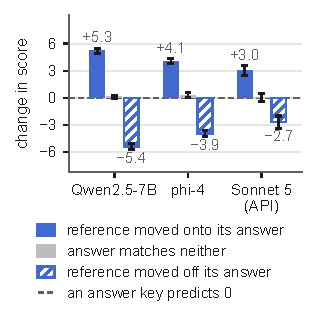
\includegraphics[width=0.40\textwidth]{figures/fig1_rotation.pdf}
\caption{\textbf{The swap over the whole replication pool.} Qwen2.5-7B, phi-4, and Sonnet~5 (API): mean change in score (points out of 10) of identical correct text when the reference moves onto its answer (120 tasks) or off it (93 tasks), and for answers that match neither reference (113 tasks; $+0.12$, $+0.30$, $+0.04$), with 95\% intervals. Pre-specified; Qwen2.5-7B uses the exact scorer (\cref{tab:rotation}).}
\label{fig:rotation-pool}
\end{figure}

We re-judged the replication pool's byte-identical samples with the reference moved to another correct answer.
Under Qwen2.5-7B,\reana{} phi-4, and Sonnet~5, text the reference moves onto gains 3 to 5 points and text it moves off loses about as much, while correct text that matches neither reference barely moves (\cref{fig:rotation-pool}).
All 12 registered cells for Qwen2.5-7B and phi-4 went as predicted; one registered prediction, that the swap would be ordered by numeric distance from the reference, failed (\cref{app:ledger}).

The swap is not an artifact of our own wording: it survives the verbatim MT-Bench template, which drops ``trusted'' and asks for an explanation first. That template also asks for a comparison, so we ran the swap again under a prompt that names the reference and never says to use it. Credit still follows the reference, where credit is a yes-or-no judgment rather than the 0--10 score above: answers that stop matching it lose 26 pp for GPT-4.1 and 13 for Sonnet~5. Text matching neither reference moves $-6$ pp for Sonnet~5, a larger move than the 5 pp we registered as a bound, and $-3$ pp for GPT-4.1, whose interval includes zero (\cref{app:r30}). Told not to compare, though, every interval includes zero for both judges (\cref{app:r31}): the effect needs no instruction to compare, and an explicit instruction against comparing removes it. On arithmetic it mostly vanishes, however, when the reference is written as an expression or hidden inside a worked solution (\cref{app:rotation,app:mechanism}).

Does the problem fade as judges improve? On arithmetic, thinking before scoring removes most of the swap (\cref{app:reasoning}). On factual questions it shrinks the effect without removing it: Sonnet~5's added false rejections fall from 36 to 15 points (\cref{app:acceptance}), and o3-mini, a reasoning model, running the HLE grader still credits almost no correct answer that differs from the reference (\cref{sec:cost}), under a grader that tells it not to argue for a different answer.

\section{Prediction 2: correct answers that differ from the reference are graded worse}
\label{sec:p2}

\begin{figure}[t]
\centering
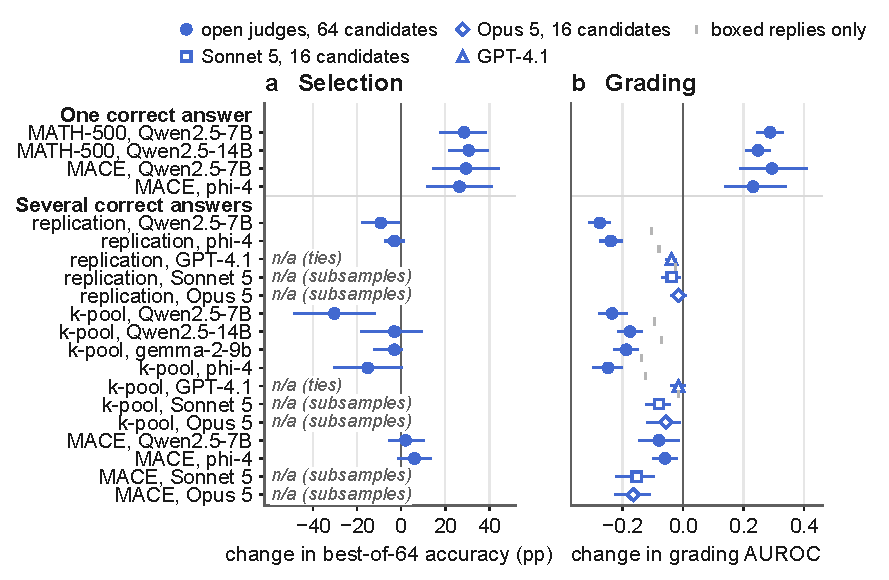
\includegraphics[width=0.86\textwidth]{figures/fig2_onevsseveral.pdf}
\caption{\textbf{With one correct answer the reference helps; with several, it lowers grading.} Change from showing the reference (referenced minus blind, per task, 95\% intervals). \textbf{(a)}~Best-of-64 accuracy; on MATH-500 the reference is the final answer alone. \textbf{(b)}~Grading AUROC. Rows marked n/a cannot be measured in that cell. Registration status per value: \cref{tab:labelings-gnm,tab:protocols}.}
\label{fig:onevsseveral}
\end{figure}

\paragraph{Several correct answers.}
The reference makes judges reject correct answers they would otherwise accept: under the registered labels, Qwen2.5-7B scores 28\% of the differing correct answers 3 or below with the reference, against 0.4\% blind\reana{} (\cref{app:grid}).
Grading suffers with it. The AUROC that separates those answers from wrong ones falls by 0.06 to 0.16 for the four judges on factual questions and by 0.17 to 0.27 for the four open judges on the constructed pools (\cref{fig:onevsseveral}b). We registered the factual falls for Qwen2.5-7B, Sonnet~5, and Opus~5 in advance; the constructed-pool falls are post hoc,\ph{} because they use the any-format labels we adopted after the registered checker proved too strict.

Relabeling moves their size, not their sign. All four open judges fall under registered, model-read, and boxed-only labels alike, and the pre-specified estimate under the registered labels, Qwen2.5-7B on the replication pool, falls by 0.29 (\cref{tab:labelings-gnm}); read the fall on boxed replies alone, 0.07 to 0.14, as the conservative bound, since the any-format labels that give the larger numbers over-credit some replies (\cref{app:grid}); \cref{app:ledger} gives every registered prediction and its outcome.

\paragraph{One correct answer.}
With one correct answer the reference helps, as P2 requires.
On MATH-500, showing only the final answer raises best-of-64 accuracy by 28.6 and 30.6~pp for Qwen2.5-7B and 14B,\reana{} as the full solution does; on \textsc{MACE}'s single-answer questions it raises accuracy by 29.4\ph{} and 26.5~pp for Qwen2.5-7B and phi-4 (\cref{fig:onevsseveral}a).

\paragraph{Verdict.}
P2 holds on factual questions for Sonnet~5, Opus~5, Qwen2.5-7B, and phi-4, and on the constructed pools for the four open judges and Sonnet~5. Two intervals include zero: GPT-4.1 on factual questions, whose falls are small everywhere, and Opus~5 on the replication pool (\cref{app:ledger}). On the constructed pools the API judges fall far less than the open judges.

Selection is less exposed than grading. Best-of-64 accuracy did not fall on \textsc{MACE}'s multi-answer questions, so our registered loss there was not confirmed, and on the $k$-pool the losses concentrate where no correct candidate matches the reference\ph{} (\cref{app:estimator}).
\section{Prediction 3: the effect persists after blind acceptance}
\label{sec:p3}

\begin{figure}[tb]
\centering
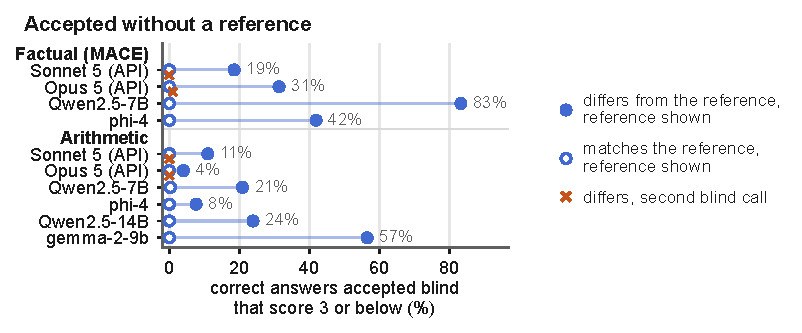
\includegraphics[width=0.88\textwidth]{figures/fig3_acceptance.pdf}
\caption{\textbf{The reference makes judges take back credit they had already given.}
Each row is one judge. We keep the correct answers it accepted with no reference in front of it, then show it the reference and count how many it now scores 3 or below. Filled circles are answers that differ from the reference, hollow circles answers that match it. Acceptance means a blind 10 for Sonnet~5 and Opus~5, and for the open judges the blind score that at most 3\% of wrong answers reach. Pre-specified: the second blind calls and Opus~5's shares; the rest is post hoc.}
\label{fig:reasoning}
\end{figure}

\paragraph{What the skeptic would say.}
So far the reference moves scores, and a skeptic can explain that away: perhaps the judge cannot tell on its own that a different answer is correct, so the reference is the only evidence it has. Call this \emph{verification failure}. If that is the whole story, the problem belongs to the model's knowledge, not to how we grade.
The explanation makes a clear prediction. Suppose a judge reads a correct answer with no reference at all and accepts it. It has just shown that it recognizes the answer as correct, so it has no reason to change its mind when a different correct answer is then shown as the reference.
The alternative is \emph{agreement}: the judge defers to whichever answer it is shown, even when it can see that the candidate is right. Agreement predicts that the judge takes the credit back.

\paragraph{What the judges do.}
An answer counts as accepted when the judge gives it a blind 10, or, for the open judges, the blind score that at most 3\% of wrong answers reach (\cref{fig:reasoning}).
On \textsc{MACE}'s multi-answer questions, Sonnet~5 and Opus~5 take back credit from 19\% and 31\% of the accepted answers that differ from the reference, and from none of the 140 that match it; the constructed pools give smaller shares (\cref{tab:r20-retest}). At the open judges' post hoc threshold, phi-4 takes back 42\% and Qwen2.5-7B 83\%, also on \textsc{MACE}.\ph{}
Verification failure predicts none of this.

\paragraph{It is not noise.}
Scores wander a little between calls, so we asked the same judges again, the same way, still with no reference.
Of the 843 accepted answers that differ from the reference, pooled over both judges, 2 fell to 3 or below on that second call. With the reference in front of them, 117 did, against none of the 383 that match it.

\paragraph{It is not our wording either.}
Asked only whether the response is correct, with no rubric of ours and no instruction about the reference, GPT-4.1 and Sonnet~5 take back credit from 22\% and 14\% of the answers they had accepted, and from none of the matching ones.\reana{}
Asked to reason first, by chain of thought, verify-first, or solve-first, they take back 1\% to 9\% (\cref{app:r27}). Those three, unlike the direct prompt, tell the judge to use the reference, and none has a second blind call to compare against.

\paragraph{Verdict.}
P3 holds for all six judges with a usable acceptance test, and on factual questions for four judges from three developers: two with the second blind call as a noise control, and two at a threshold we chose after seeing the data.
Verification failure alone therefore cannot explain the effect, although it may explain part of it for some judges.
Accepting an answer blind is a proxy for verifying it, not proof: a judge can accept an answer without checking it, and Opus~5 gives a blind 10 to 5\% to 8\% of wrong answers (\cref{app:acceptance}) --- a band that covers its own 2.7\% to 4.7\% retraction on the constructed pools, though not Sonnet~5's 8.7\% and 14.9\% there.
And agreement, as we have defined it, still covers a judge that simply assumes the question has one intended answer; P3 does not separate that from rewarding a match.

\section{How much it matters, and what sets the size}
\label{sec:cost}

\begin{figure}[tb]
\centering
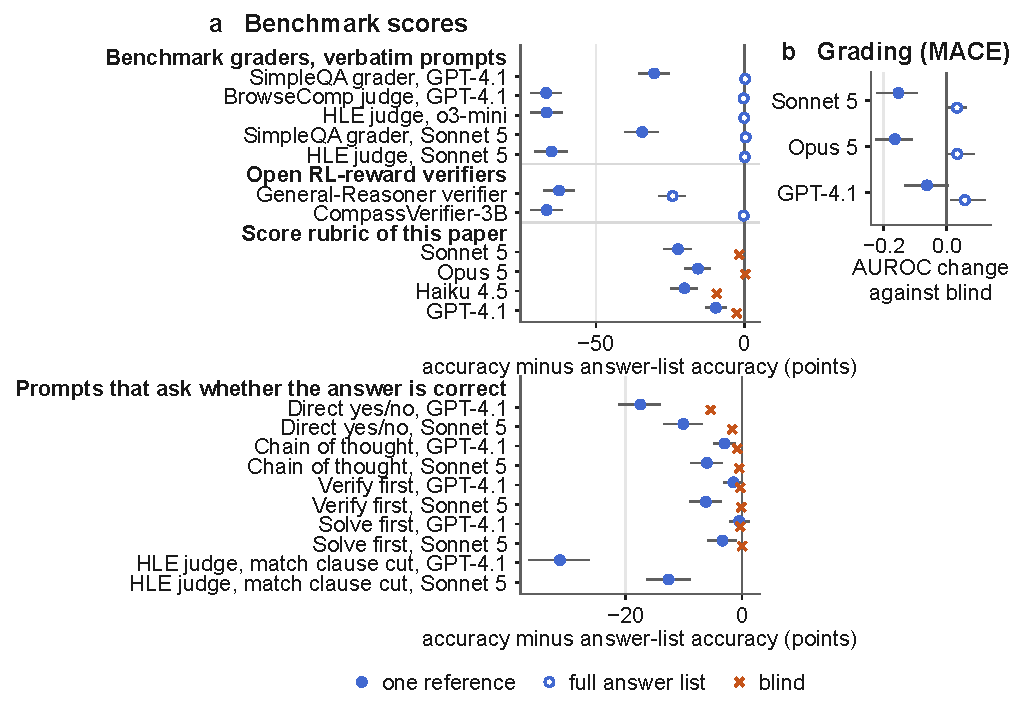
\includegraphics[width=0.85\textwidth]{figures/fig4_graders.pdf}
\caption{\textbf{Graders told to match under-count correct answers.} Asking whether the answer is correct shrinks the gap; giving the grader every correct answer closes it for all but one verifier.
\textbf{(a)}~Four models answered 149 \textsc{MACE} questions that have several correct answers. Each marker shows how far a grader's accuracy falls below \emph{answer-list accuracy}, the accuracy scored against the full lists, when the grader sees one reference drawn at random. The benchmark graders run exactly as shipped, each with the judge it is configured to use (GPT-4.1, or o3-mini for HLE). The lower panel, on a narrower scale, asks the same judges whether the answer is correct.
\textbf{(b)}~What the reference does to grading on the 40-task \textsc{MACE} subsample: the change in how well each judge separates correct answers that differ from the reference from wrong ones. 95\% intervals; every value was pre-specified.}
\label{fig:graders}
\end{figure}

\paragraph{Graders shipped with benchmarks.}
We took one answer from each of Llama-3.1-8B-Instruct (its first stored sample), Claude Haiku~4.5, Sonnet~5, and Opus~5 to each of 149 \textsc{MACE} questions with several correct answers.
Every answer was graded with the SimpleQA grader and the judge shared by BrowseComp and HLE, copied from their repositories and run as configured there (GPT-4.1 for SimpleQA and BrowseComp, o3-mini for HLE), and with Sonnet~5 (\cref{app:r24}).
Each grader saw one reference, drawn at random from the answer list.
The SimpleQA grader credits 47\% to 53\% of the correct answers that differ from it, so accuracy falls 30 to 34 points below answer-list accuracy. The BrowseComp/HLE judge credits 0\% to 2.3\%, and accuracy falls 65 to 67 points (\cref{fig:graders}a).
Two open RL-reward verifiers do the same: given one reference, General-Reasoner's verifier and CompassVerifier-3B credit 6\% and 0\% of these answers (\cref{app:r26}).
Our own score rubric, with four judges, leaves the models 10 to 22 points below the answer lists (\cref{app:acceptance}).
Choosing the reference rather than drawing it shrinks the shortfall without removing it: given the answer most of the four models produce, which is the best case for the grader, the SimpleQA grader falls 9 points short and the HLE judge 20; given \textsc{MACE}'s own first-listed answer, 26 and 56. Only one of the four reductions has an interval that includes zero: the SimpleQA grader's, under the first-listed rule. The HLE judge credits none of the answers that differ from its reference under either rule, so its gap narrows almost entirely because fewer answers differ (\cref{app:r30}).

\paragraph{Who should care: reuse across a capability boundary.}
These graders are right for the benchmarks they were written for.
By adjudicated LLM labels, 0\% to 3\% of sampled SimpleQA, BrowseComp, and HLE questions have several correct answers (\cref{app:prevalence}), so their own leaderboards are probably little affected. Read that as a lower bound: adjudication stopped at a spending cap and the disagreements left over kept the conservative label, and HLE alone reaches 6.0\% if six of them go the other way.
The failure is reuse across a capability boundary: a grader written for questions beyond its judge, pointed at questions it can answer (\cref{sec:fix}). We offer that as a reading, not an isolated variable: our two settings differ in difficulty and in the number of correct answers at once, and the shortfall below needs only the second.
General-Reasoner's single-reference verifier rewards an RL training set~\citep{ma2025generalreasoner} in which 5.5\% of questions admit several answers after adjudication, 18\% by either annotator, and 30\% to 44\% of sampled NQ-open questions do.\ph{}
Reward signals are the larger risk, since there the judge shapes a policy rather than reporting a score, and both verifiers above were built for RL rewards.
We therefore state this as a concern rather than a demonstrated harm.

\paragraph{What sets the size.}
Told to ``focus only on whether the answers match'', the HLE judge credits almost no differing correct answer, even with o3-mini (\cref{fig:graders}a, lower panel; \cref{app:r25,app:r26}).
Removing that match clause and adding that a different correct answer is correct recovers 35 points for GPT-4.1 and 53 for Sonnet~5, but leaves 31 and 13, outside our registered bound.
Asked instead whether the response is a correct answer, GPT-4.1 and Sonnet~5 fall 17 and 10 points short, against 5 and 2 blind; asked to reason first, 0.5 to 6 points, which closes most of GPT-4.1's gap but, by our registered test, not Sonnet~5's.

\section{How to fix it}
\label{sec:fix}

\paragraph{Give the judge every correct answer.}
An answer key is the reading under which the reference is harmless.
Stated as ``any one of the following is a complete correct answer'', the full answer list brings all five benchmark-grader configurations within 0.5 points of the answer lists and raises their credit for differing correct answers to 99\% or more (\cref{fig:graders}a).
That agreement is partly by construction, since the same lists define correctness: what it shows is that the graders follow a list when given one, admitting at most 3 of 56 more wrong answers.
Our registered bound of 3 points on that extra credit still failed for the BrowseComp/HLE judge with GPT-4.1 and o3-mini.
With our rubric the list also repairs grading: AUROC is 0.03 to 0.06 above blind for Sonnet~5, Opus~5, and GPT-4.1, although Opus~5's interval touches zero (\cref{fig:graders}b; \cref{app:r24}).
The list fixes CompassVerifier-3B but not General-Reasoner's 1.5B verifier, which credits 67\% of differing correct answers with the list but also 30\% of wrong ones (\cref{app:r26}).
A list is still closed: whether it makes judges reject correct answers it omits is untested, and lists can be incomplete (\cref{app:mace}).

\paragraph{When the answers cannot be listed.}
If the judge can answer the questions, remove any instruction to match and ask whether the answer is correct.
We compared three such prompts on the 40-task \textsc{MACE} subsample, which has many wrong answers.
Letting the judge solve the question first had the smallest grading loss: AUROC $-0.04$ and $-0.05$ against blind, with wrong answers wrongly credited up by at most 3.2 points.
It still rejected 5 to 7 points more of the differing correct answers (\cref{app:r26}).
Telling the judge that any correct answer deserves full credit helps but does not suffice: added to our rubric, it cuts the rise in false rejections on \textsc{MACE} from 36 to 18 points for Sonnet~5 and to 8 for Opus~5 (\cref{app:acceptance}).
Forbidding comparison works better still: accuracy comes within 1.7 points of the lists, though GPT-4.1 then credits 20\% of wrong answers against 7\% (\cref{app:r31}). Read accuracy here with its pool in mind: 90.6\% of these answers are correct, so it tracks recall and hides that cost, which a pool with more wrong answers would expose.
One protocol we registered did not help: scoring blind and then rescoring with the reference left grading below blind for most open judges\ph{} (\cref{app:mitigation}).

\paragraph{Questions beyond the judge.}
On such questions, the instruction to match can be what keeps wrong answers out.
We took the 200 HLE questions of our prevalence audit (6 labeled as having several answers, 53 unclear; \cref{app:prevalence}) and graded two models' answers to them; HLE's official judge marks almost all of them wrong.
With the reference, GPT-4.1 credited 17\% of those answers under the direct prompt and 26\% when it solved first, often after calling the reference wrong.\ph{}
Sonnet~5 credited at most 1\% (\cref{app:r27}).
A change of instruction is therefore safe only for the judges and questions on which it has been checked.

\paragraph{A recipe.}
\begin{itemize}[leftmargin=1.2em,itemsep=0pt,topsep=1pt,parsep=0pt]
\item \textbf{Answers that can be listed:} give the grader every one, and check that a trained verifier follows lists; one of our two did not.
\item \textbf{No list and no checker:} if the judge can answer the questions, ask whether the response is correct rather than telling it to match; if not, keep the match instruction and first check that the judge does not overrule the reference on known wrong answers.
\item \textbf{Audit:} score a sample blind as well and read answers accepted blind but rejected with the reference.
\end{itemize}

\section{Related work}
\label{sec:related}

\paragraph{Reference-guided judging.}
References are the standard remedy for grading math and reasoning with LLM judges~\citep{zheng2023judging,refguided2024,chen2026rethinking}, and judges without them over-credit wrong answers~\citep{generous2026}. Judge models, benchmark graders, and answer matching all check a response against one gold answer~\citep{zhu2023judgelm,kim2024prometheus,wei2024simpleqa,wei2025browsecomp,phan2025hle,chandak2025answermatching}, as do RL-reward verifiers~\citep{chen2025xverify,liu2025compassverifier,yan2025verifybench}; false negatives from rule-based checking slow RL~\citep{xu2025tinyv,huang2025pitfalls}.
Judges depend on the reference being correct~\citep{judgingref2026,krumdick2025nofreelabels}, diverge from humans under reference-based grading~\citep{thakur2024judging}, and favor the reference's solution method~\citep{fixation2025}.

\paragraph{Single references and many correct answers.}
Translation metrics reward outputs resembling the particular reference, and open-domain question answering has long under-credited correct answers missing from a gold list, which answer-equivalence methods and multi-answer benchmarks target~\citep{min2020ambigqa,kamalloo2023evaluating,amouyal2022qampari,li2024pedants}; on our constructed tasks the list is complete and the judge still favors the one answer it is shown (\cref{app:relatedbias}).

\paragraph{Judge biases and optimization.}
Known judge biases concern position, length, self-preference, and a shown \emph{score}; none varies which correct answer is shown, and the effect here resembles sycophancy except that the suggestion is correct (\cref{app:relatedbias}).

\section{Limitations}
\label{sec:limits}

\textbf{Labels.} Any-format labels were checked by a frontier model, not by humans, and boxed replies alone give conservative estimates; prevalence labels come from LLM annotators with low agreement ($\kappa \le 0.35$), and HLE labels from HLE's own judge, which credits none of the differing correct answers we measure, so some we count as wrongly accepted may be valid alternatives (\cref{app:r27}).
\textbf{Tasks.} Constructed pools come from five arithmetic families and one generator, natural data from two \textsc{MACE} domains. The benchmark study uses one answer per model, with references drawn at random and, in \cref{app:r30}, chosen; three graders grade their own answers (\cref{app:acceptance}), and intervals resample questions, not grader calls. Open-ended tasks (summarization, writing, agent trajectories) are untested. Our exploratory preference-training runs were inconclusive, so harm to RL training is not demonstrated (extended appendix).
\textbf{Judges, prompts, and registration.} Open judges have at most 14B parameters, our wordings do not exhaust reference prompts, the correctness prompts were tested for two judges, and only the API judges have a second blind call as a noise control, which the round-30 and round-31 swaps lack. Whether a judge with tools or retrieval anchors the same way is untested (\cref{app:frontier}). No experiment manipulates verification directly, and most registrations are timestamped commits with a verdict rule adopted afterwards (\cref{app:ledger}).

\subsection*{AI use statement}
Generative AI models were the experimental subjects: open and frontier LLMs generated candidate answers and served as the judges and verifiers under study (\cref{sec:setup}, \cref{app:setup}); three Claude models answered the benchmark questions of \cref{sec:cost}, which Claude models, GPT-4.1, and o3-mini graded; GPT-4.1-mini and Claude Haiku~4.5 answered the HLE questions of \cref{sec:fix}, which o3-mini labeled; and Claude Opus~5 read replies for the label audit. One pilot in the extended appendix used a Claude model to generate candidate solutions, each verified by exact checks, and Qwen2.5-14B read unboxed replies for one labeling. We used generative AI tools to help write analysis code, draft and edit text, produce figures, search and verify related work, audit the preregistration ledger, and label samples of dataset questions for two prevalence audits, the first with two passes from one model family and the second with Claude Sonnet~5 and GPT-5-mini adjudicated by Claude Opus~5; no label was checked by human annotators. Every number in the paper is produced by committed analysis scripts from stored model outputs, and we checked every quoted number against those outputs. We take responsibility for the final content of this work.

\subsection*{Ethics statement}
This work studies a failure of automated evaluation that can make models look worse than they are on questions with several correct answers. We release no new model and no attack on a deployed system. The findings raise a concern for pipelines that use reference-guided judges as reward signals on such questions, which may reward matching the reference rather than being correct; our exploratory training runs were inconclusive and did not show a policy learning to copy the reference (extended appendix in the supplement). No human subjects were involved.

\subsection*{Reproducibility statement}
\Cref{app:setup} and the appendices it cites specify the judges, prompts, and scorers, and \cref{app:ledger} gives the verdict totals and every registered prediction that was not confirmed; the extended appendix in the supplement tabulates every pool and lists every prediction with its registration type and outcome. The anonymized supplementary material contains task generators and checkers, candidate pools, the answer labelings, all judge score files, the analysis scripts that produce every number, table, and figure, an extended appendix, and the registration documents with commit hashes replaced by stable tokens.

\bibliography{references}
\bibliographystyle{iclr2027_conference}

\newpage
\appendix
\crefalias{section}{appendix}
% Condensed appendix for main.tex (v3). The complete appendix is appendix_extended.tex, compiled by extended_appendix.tex
% into extended_appendix.pdf for the supplement. Every number here is copied from it; tables in tables/ are generated by
% scripts/make_tables.py from papers/analysis/*.json.

\section*{Appendix overview}
Each section below supports the main-text sections listed. The extended appendix in the supplementary material contains every analysis and the full ledger, including exploratory work that is not part of the paper's claims (preference-training runs, a constraint-problem pilot, code experiments, and composition studies).

\begin{center}
\footnotesize
\setlength{\tabcolsep}{4pt}
\renewcommand{\arraystretch}{1.08}
\begin{tabular}{cL{10.6cm}c}
\toprule
& Contents & Main text \\
\midrule
\ref{app:setup} & Pools, prompts and the conditions each is used in, why the default rubrics invite comparison, the Figure~1 example & \ref{sec:intro}, \ref{sec:setup} \\
\ref{app:survey} & Graders, libraries, RL pipelines, and papers that grade against one reference, and what their prompts say & \ref{sec:intro} \\
\ref{app:prevalence} & How often questions admit several answers in nine datasets (LLM labels) & \ref{sec:cost}, \ref{sec:fix} \\
\ref{app:ledger} & Verdict totals and every registered prediction that was not confirmed & all \\
\ref{app:mace} & \textsc{MACE} domains, answer-list completeness, and answer matching & \ref{sec:setup}, \ref{sec:fix} \\
\ref{app:grid} & Answer labelings, the label audit, and grading under each labeling & \ref{sec:setup}, \ref{sec:p2} \\
\ref{app:estimator} & Exact scorer, bare-answer reference on MATH-500, and selection & \ref{sec:setup}, \ref{sec:p2} \\
\ref{app:reasoning} & Reasoning and thinking judges & \ref{sec:setup}, \ref{sec:p1} \\
\ref{app:rotation} & Swap test: all cells, the MT-Bench template, and the pool-level plot & \ref{sec:p1} \\
\ref{app:mechanism} & How the form of the reference (expression, masked solution) changes its pull & \ref{sec:p1} \\
\ref{app:frontier} & Frontier API judges on 16-candidate subsamples & \ref{sec:p2} \\
\ref{app:acceptance} & Blind acceptance and a second blind call, the full-credit sentence, benchmark scores with our rubric, and a second reference draw & \ref{sec:p1}, \ref{sec:p3}, \ref{sec:cost} \\
\ref{app:r24} & Benchmark graders run verbatim, and the full answer list & \ref{sec:cost}, \ref{sec:fix} \\
\ref{app:r25} & Judges that reason before deciding & \ref{sec:cost} \\
\ref{app:r26} & Direct prompt, edited HLE judge, grading with many wrong answers, and open RL-reward verifiers & \ref{sec:cost}, \ref{sec:fix} \\
\ref{app:r27} & P3 under correctness prompts, and hard single-answer questions & \ref{sec:p3}, \ref{sec:fix} \\
\ref{app:mitigation} & Blind-then-reveal, the max rule (post hoc), and other mitigations & \ref{sec:p2}, \ref{sec:fix} \\
\bottomrule
\end{tabular}
\end{center}

%==========================================================================================
\FloatBarrier
\section{Setup details}
\label{app:setup}

Every number in this condensed appendix also appears in the extended appendix. The ledger keeps the names used in the registrations, calling the swap test \emph{rot\-ation} and the margin the \emph{an\-choring margin}; the two rubric wordings are $a$ and $b$.

\paragraph{Pools.}
The pools are summarized in \cref{sec:setup}, and the extended appendix tabulates each with its generator and judges. The benchmark answers are one answer per model from Llama-3.1-8B-Instruct, Haiku~4.5, Sonnet~5, and Opus~5 to 149 \textsc{MACE} questions with several correct answers (596 answers). \paragraph{Scoring.}
Open judges run in vLLM at temperature 0 and produce at most four tokens. We read the top-20 log-probabilities of the first generated token and take the probability-weighted mean over the score tokens 0 to 10, renormalized over their captured probability. Qwen2.5, gemma-2, and Mistral write ``10'' as the two tokens ``1'' and ``0''; the original scorer assigned all probability on ``1'' to 10 or to 1 according to the greedy reply, and the pre-specified exact scorer of \cref{app:estimator} runs one more forward step to split it. Mistral-7B's tokenizer has no single-token digits, so its scores are the integers parsed from its greedy replies. Sonnet~5 through the Anthropic API ran with extended thinking disabled and returns its score through a forced, schema-validated tool call; GPT-4.1 uses the same expected-score estimator as the open judges, but its API returns at most five alternatives per token.

\paragraph{Measures.}
For each task we select the sample with the highest rubric-$a$ score; when several samples tie at the maximum, accuracy is the mean validity of the tied samples. False rejection uses rubric-$a$ scores of oracle-valid samples whose extracted answer (the last \texttt{\textbackslash boxed\{\}} content, loosely normalized, or the whole reply if there is none) differs from the reference. Both are averaged per task and bootstrapped over tasks (1,000 resamples). The anchoring \emph{margin} is the mean score of valid samples that match the reference minus the mean score of valid samples that do not. \emph{Inflation}, the endpoint of the early registered experiments, is the standardized rubric-$b$ score of the selected sample minus the mean standardized rubric-$b$ score of samples with the same validity, against a permutation null, on tasks with pass rate in $[0.2, 0.8]$, and reported as the referenced-minus-blind difference per task; the extended appendix gives the full definition.

\paragraph{Score rubrics and the conditions that use them.}
The judge receives a system message with the rubric and a user message containing ``Problem:'', optionally ``Reference answer (trusted):'', and ``Candidate solution:'' followed by ``Score:''. \emph{Blind condition:}
\begin{quote}\small
(a) You are a strict grader. Read the question and the candidate response. Rate how correct and appropriate the response is on a scale from 0 (completely wrong or off-task) to 10 (fully correct). Judge the content, not the writing. Respond with only the integer score.\\[2pt]
(b) Evaluate the following response for correctness. Consider whether it actually answers the question asked. Ignore presentation quality. Give a single number from 0 to 10, where 0 means entirely incorrect and 10 means fully correct. Output only that number.
\end{quote}
\emph{Referenced condition} (the default whenever a reference is shown):
\begin{quote}\small
(a) You are a strict grader. You are given a question, a reference answer known to be correct, and a candidate response. Rate the candidate's correctness on a scale from 0 (completely wrong) to 10 (fully correct), using the reference to check it. Judge the content, not the writing. Respond with only the integer score.\\[2pt]
(b) Compare the candidate response against the trusted reference answer provided. Score how correct the candidate is, from 0 (entirely incorrect) to 10 (fully correct). Presentation does not matter. Output only a single number.
\end{quote}
\emph{Mitigation conditions only.} The full-credit sentence and the second instruction wording each append one of these sentences to the referenced rubric:
\begin{quote}\small
Note: the reference shown is one valid answer among possibly many; the question may have several correct answers, and any correct answer deserves full credit even if it differs from the reference.\\[2pt]
Important: do not compare the candidate's answer to the reference. Use the reference only to understand the problem. Verify the candidate's answer on its own merits; a correct answer that differs from the reference must receive the same score as one that matches it.
\end{quote}
\emph{Blind-then-reveal condition.} The first call scores the candidate with the blind rubric. The second call appends to the referenced rubric: ``You have already assessed this candidate without seeing any reference. A correct answer that differs from the reference must keep the score you gave it; revise only if the reference reveals the candidate is actually wrong.'' Its user message shows the reference as ``Reference answer (one valid answer, trusted)'' and ends with ``Your blind score for this candidate was $x$ out of 10.''

\paragraph{What the default referenced rubrics ask.}
Both default referenced rubrics invite comparison with the reference: rubric~$a$ asks the judge to use the reference to check the candidate, and rubric~$b$ begins ``Compare the candidate response against the trusted reference answer provided.'' Neither says that a question can have several correct answers. The sentence ``the reference shown is one valid answer among possibly many'' is not part of either default rubric; it defines a separate mitigation condition, reported as such (\cref{app:acceptance,app:r24,app:mitigation}). A judge that follows the comparison instruction could therefore favor the reference because it was told to. The effect does not rest on our wording. It appears under the verbatim MT-Bench single-answer template (\cref{app:rotation}), which also asks for a comparison with the reference; under a direct prompt that asks only whether the response is correct and says nothing about how to use the reference (\cref{app:r26}); under chain-of-thought, verify-first, and solve-first prompts that ask the judge to use or check the reference, although reasoning shrinks it (\cref{app:r25}); for correct answers the judge had already accepted blind (\cref{app:acceptance}); and, under correctness prompts, for answers credited blind (\cref{app:r27}). The wording does change its size (\cref{app:r26}).

\paragraph{Other prompts.}
The benchmark graders are copied verbatim from their repositories (\cref{app:r24}); the direct, chain-of-thought, verify-first, and solve-first prompts are quoted in \cref{app:r25,app:r26}; the open RL-reward verifiers use their own templates (\cref{app:r26}).

\paragraph{The Figure 1 example.}
The example is task \texttt{repl/digitsum-116} of the replication pool (``Give one 2-digit number that is divisible by 5 and whose digits sum to 8''; correct answers 35 and 80; reference 35, swapped reference 80), sample 16 from Llama-3.1-8B-Instruct, scored by Qwen2.5-7B with the exact scorer. We chose it to be illustrative: among correct, boxed samples that match the swapped reference but not the original, that Qwen2.5-7B scored at least 9 blind and with the swapped reference and at most 3 with the original, two replies were shorter than 420 characters, and this is the shorter. Its swap (6.4 points) is larger than the pool average (\cref{fig:rotation-pool}). The full reply:
\begin{quote}\small
To find a 2-digit number that is divisible by 5, the ones digit must be either 0 or 5.\\[2pt]
Let's consider the case where the ones digit is 0. In this case, the tens digit must be 8 for the digits to sum to 8. The number would be 80.\\[2pt]
Now, let's check if 80 is divisible by 5. Since $80 \div 5 = 16$, 80 is indeed divisible by 5.\\[2pt]
The number 80 meets the given conditions, so we can stop here.\\[2pt]
The answer is \texttt{\textbackslash boxed\{80\}}.
\end{quote}

%==========================================================================================
\FloatBarrier
\section{How widely graders rely on one reference}
\label{app:survey}

We surveyed benchmarks whose official scorer is an LLM judge, evaluation libraries and cloud platforms with a built-in correctness judge, RL reward pipelines that use an LLM verifier, and research papers from 2023 to 2026 that evaluate or train with an LLM judge. Every entry was checked on 14 September 2026 against its primary source (repository code at a pinned commit, official documentation, or the paper); the records, 24 verbatim judge templates, and all quotes are in the supplementary material. An entry counts as \emph{reference-guided} when the judge sees one gold answer, or a closed list of them, and decides correctness from it (\cref{tab:survey}).

\begin{table}[htbp]
\centering
\caption{Surveyed graders that give an LLM judge one reference answer or a closed list of them. Research papers were selected because they use such a judge; 10 checked candidates that did not were dropped. Partly: Arize Phoenix (reference template only in an older release) and Rubrics as Rewards (references write the rubrics).\ph}
\label{tab:survey}
\footnotesize
\setlength{\tabcolsep}{3pt}
\begin{tabular}{L{2.2cm}ccL{7.8cm}}
\toprule
Group & Surveyed & One reference & Reference-guided entries \\
\midrule
Benchmarks & 16 & 11 & SimpleQA~\citep{wei2024simpleqa}, SimpleQA Verified~\citep{haas2025simpleqaverified}, BrowseComp~\citep{wei2025browsecomp}, HLE~\citep{phan2025hle}, the simple-evals MATH checker~\citep{simpleevals}, MT-Bench~\citep{zheng2023judging}, FreshQA~\citep{vu2023freshllms}, CRAG~\citep{yang2024crag}, MixEval~\citep{ni2024mixeval}, Omni-MATH~\citep{gao2024omnimath}, FRAMES~\citep{krishna2025frames}. Not: TruthfulQA, HealthBench, GAIA, LiveBench, Arena-Hard \\
Evaluation libraries & 12 & 11 + 1 partly & Inspect AI~\citep{inspectai}, OpenAI Evals~\citep{openaievals}, LangChain~\citep{langchainevals}, openevals~\citep{openevals}, LlamaIndex~\citep{llamaindexcorrectness}, RAGAS~\citep{es2023ragas}, DeepEval~\citep{deepeval}, MLflow~\citep{mlflowjudges}, promptfoo~\citep{promptfoofactuality}, TruLens~\citep{trulens}, OpenCompass~\citep{opencompassjudge}; Phoenix~\citep{phoenixevals} partly \\
Cloud platforms & 4 & 3 & OpenAI graders~\citep{openaigraders}, Azure AI Foundry~\citep{azurefoundrysimilarity}, AWS Bedrock~\citep{bedrockjudgeprompts}. Not: Vertex AI \\
RL reward pipelines & 11 & 10 + 1 partly & DeepSeek-R1~\citep{deepseek2025r1}, Kimi k1.5~\citep{kimi2025k15}, Qwen3~\citep{yang2025qwen3}, Seed1.5-Thinking~\citep{seed2025thinking}, General-Reasoner~\citep{ma2025generalreasoner}, RLVR across domains~\citep{su2025rewardbridge}, xVerify~\citep{chen2025xverify}, CompassVerifier~\citep{liu2025compassverifier}, TinyV~\citep{xu2025tinyv}, OpenAI reinforcement fine-tuning~\citep{openairft}; Rubrics as Rewards~\citep{gunjal2025rar} partly \\
Research papers, 2023--2026 & --- & 34 & Math and science~\citep{huang2025pitfalls,chernyshev2024umath,lu2025ineqmath,xu2025ugphysics,minimax2025m1,cheng2025guru,bercovich2025llamanemotron,huang2024olympicarena,fang2024mathodyssey}; proofs and competition grading~\citep{petrov2025proofbluff,luong2025imobench,mahdavi2025refgrader,balunovic2025matharena}; code~\citep{zhuo2024icescore,tong2024codejudge}; QA and RAG~\citep{chandak2025answermatching,he2024chinesesimpleqa,ru2024ragchecker,rau2024bergen,refguided2024,kamalloo2023evaluating,thakur2024judging,wang2023evouna}; agents and deep research~\citep{wu2025webwalker,zhou2025browsecompzh,wu2025webdancer,li2025websailor,gao2025asearcher,zheng2025deepresearcher,chen2025browsecompplus,du2025deepresearchbench,li2025webthinker,liu2025webexplorer,tongyi2025deepresearch} \\
\bottomrule
\end{tabular}
\end{table}

\paragraph{What the prompts say.} We could read 34 judge prompts in full (a different set from the 34 research papers). Of these, 27 define correctness as matching the reference, 4 partly, and 3 offer it only as an aid. Two say that several answers can be valid, and both give the judge a closed list~\citep{ni2024mixeval,vu2023freshllms}; three more allow different wording but require the reference's content. None tells the judge to credit a correct answer outside the reference. Five declare the reference correct: ``Take it as granted that the Ground Truth is always correct'' (CRAG), ``The reference answer is ALWAYS correct'' (Omni-MATH), ``THE STANDARD ANSWER IS ALWAYS CORRECT AND THE QUESTION IS PERFECTLY VALID. NEVER QUESTION THEM'' (CompassVerifier), ``You can assume that the standard answer is definitely correct'' (OpenCompass), and the HLE and BrowseComp judge's ``precise and unambiguous [correct\_answer]''. Reward prompts follow the same pattern: DeepSeek-R1's reward prompt rates an answer correct when it ``fully aligns with the reference answer''~\citep{deepseek2025r1}.

\paragraph{Research papers.} Eight of the 34 papers use the judge as an RL reward or data filter. In seven others, all evaluations, the tasks admit several valid answers and the judge still sees one reference or a closed list~\citep{kamalloo2023evaluating,wang2023evouna,zheng2025deepresearcher,du2025deepresearchbench,zhuo2024icescore,tong2024codejudge,petrov2025proofbluff}; among them, providing reference code made all three LLM-based evaluators worse on CoNaLa~\citep{tong2024codejudge}. IMO-ProofBench's grader is told the reference ``demonstrates one valid approach'' and is reported to be ``prone to be overly punitive'' for unconventional correct solutions~\citep{luong2025imobench}.

%==========================================================================================
\FloatBarrier
\section{How common are questions with several valid answers?}
\label{app:prevalence}

We sampled 200 questions (seed 0) from each of four datasets that ship one reference answer per question and labeled each as having multiple non-equivalent valid answers, a unique answer up to equivalence, or unclear. Equivalent forms of one answer (for example $1/2$ and $0.5$) count as unique, and ``find all'' questions whose answer is a single set count as unique. Each item was labeled twice independently by LLM annotators (Claude models) that did not see each other's labels, and disagreements were adjudicated by re-reading the item. Every alternative answer given for a math item was checked by computation. Both passes come from one model family, so agreement may overstate reliability, and we did not validate the labels against human annotators.
In this first audit (table in the extended appendix), curated math sets are almost entirely single-answer; the multi-answer math items are mostly underspecified problems rather than requests for an example. In NQ-open, 30.0\% of questions admit several correct answers, and 18.5\% after excluding questions whose answer changed over time.

\paragraph{Benchmarks graded against one reference, and a second annotator family.} A pre-specified extension (protocol committed before any labeling call) sampled 200 questions each from SimpleQA~\citep{wei2024simpleqa}, BrowseComp~\citep{wei2025browsecomp}, text-only exact-answer HLE questions~\citep{phan2025hle}, TriviaQA~\citep{joshi2017triviaqa}, and the WebInstruct-verified RL training set~\citep{ma2025generalreasoner}, with the definitions above. Two annotators from different developers labeled every item independently, Claude Sonnet~5 and GPT-5-mini; Claude Opus~5 adjudicated disagreements until its spending cap, after which the remaining 135 disagreements (106 on BrowseComp, most about whether an item needs deep solving) kept the conservative label (\cref{tab:prevalence-v2}); the fallback can only lower the count of questions with several answers, and had the six HLE fallbacks that involve that label gone the other way, HLE would reach 6.0\%. Questions written for a single answer rarely admit several: 0\% to 4\%. The RL training set reaches 5.5\%, and 18\% by either annotator. Agreement between the two annotators is low ($\kappa \le 0.35$ on the several-versus-other label), so these rates are rough; none was checked by humans. A GPT-5-mini relabel of the first audit's 800 items agrees with its final labels at $\kappa = 0.53$ on the several-versus-other label and marks more items as having several answers (87 of 200 NQ-open questions, against 60), so the first audit's rates are likely low.

\begin{table}[htbp]
\centering
\caption{Share of sampled questions with several valid answers after adjudication (95\% Wilson interval), agreement between the two annotators on the several-versus-other label, and the share labeled several by both and by either annotator. 200 questions per dataset; LLM annotators, not humans.\pre}
\label{tab:prevalence-v2}
\footnotesize
\begin{adjustbox}{max width=\linewidth}\begin{tabular}{lrrrrcccc}
\toprule
Dataset & $n$ & Several & Unique & Unclear & Several (\%) & $\kappa$ & Both (\%) & Either (\%) \\
\midrule
SimpleQA & 200 & 2 & 197 & 1 & 1.0 {\scriptsize$[0.3,3.6]$} & 0.00 & 0.0 & 1.5 \\
BrowseComp & 200 & 0 & 92 & 108 & 0.0 {\scriptsize$[0.0,1.9]$} & --- & 0.0 & 0.0 \\
HLE (text, exact answer) & 200 & 6 & 141 & 53 & 3.0 {\scriptsize$[1.4,6.4]$} & 0.10 & 1.0 & 15.0 \\
TriviaQA & 200 & 8 & 192 & 0 & 4.0 {\scriptsize$[2.0,7.7]$} & 0.29 & 1.5 & 8.0 \\
WebInstruct-verified (RL) & 200 & 11 & 173 & 16 & 5.5 {\scriptsize$[3.1,9.6]$} & 0.35 & 4.5 & 18.0 \\
\bottomrule
\end{tabular}
\end{adjustbox}
\end{table}

%==========================================================================================
\FloatBarrier
\section{Preregistration ledger}
\label{app:ledger}

Every confirmatory prediction was committed before its analysis was run, and for new model calls before the data existed; the verdict rule applied to them was adopted afterwards (below). Three experiments were registered on OSF with third-party timestamps\osf{} (links withheld for review; anonymized copies are in the supplementary material). The rest were committed to the project repository with a timestamp that predates the analysis\pre. Some of these rescored or re-analyzed outputs whose direction of effect was already known, such as the exact scorer (\cref{app:estimator}); the main text marks them with $\ddagger$ and this appendix labels them \pre. Analyses marked post hoc\ph{} carry no registration weight.

Verdicts follow one rule. \emph{Confirmed} means the 95\% interval excludes zero in the predicted direction, or a registered point prediction holds. \emph{Not confirmed} means the interval includes zero. \emph{Falsified} means the interval excludes zero in the opposite direction, or a point prediction fails. The rule was written into a registration made partway through the project for later experiments, and applied retroactively to all earlier predictions after most of their outcomes were known; several predictions that the registration documents mark as falsified are therefore reported here as not confirmed. The re-derivation moved predictions in both directions. Seven moved from falsified to not confirmed (P-R2B1 to P-R2B3, P-R3D1, P-R3D2, P-2D2, and the Qwen2.5-7B cell of P-RC1). Ten moved against us: P-M2 and P-S5 to falsified, P-FM3 from confirmed to falsified, P-S2, P-MC2, and P-EX2 to split, and P-FR1, P-FK2, P-SC1, and P-SC2 from confirmed to not evaluable.

A round is one dated batch of registered experiments; the registration documents in the supplement are numbered by round. Counting each registered prediction once, and from round 19 on once per judge or grader configuration, \cref{tab:ledger-totals} gives the totals. A prediction registered for several judges or training arms that got different verdicts across them is \emph{split}. \Cref{tab:ledger-failures} lists every prediction that was not confirmed, falsified, split, not evaluable, or not scored, and the excluded check; the extended appendix lists every registered experiment, including those whose predictions were all confirmed.

\begin{table}[htbp]
\centering
\caption{Registered predictions by verdict.}
\label{tab:ledger-totals}
\footnotesize
\begin{tabular}{lcc}
\toprule
Verdict & Through round 26 & Round 27 (\cref{app:r27}) \\
\midrule
Confirmed & 202 & 11 \\
Not confirmed & 14 & 0 \\
Falsified & 34 & 3 \\
Split & 17 & 0 \\
Not evaluable & 18 & 0 \\
Not scored & 2 & 0 \\
Excluded (\cref{app:frontier}) & 3 & 0 \\
\midrule
Total & 290 & 14 \\
\bottomrule
\end{tabular}
\end{table}

{\footnotesize
\setlength{\tabcolsep}{4pt}
\begin{longtable}{L{3.5cm}L{9.5cm}}
\caption{Every registered prediction that was not confirmed, falsified, split, not evaluable, or not scored, by experiment. Counts in parentheses where one entry covers several predictions. The rows contain 14 not confirmed, 37 falsified, 17 split, 18 not evaluable, and 2 not scored predictions, and the 3 excluded ones.}\label{tab:ledger-failures}\\
\toprule
Experiment & Predictions and outcome \\
\midrule
\endfirsthead
\multicolumn{2}{l}{\small\emph{\cref{tab:ledger-failures}, continued}} \\
\toprule
Experiment & Predictions and outcome \\
\midrule
\endhead
\bottomrule
\endfoot
$k$-pool and mitigations\osf{} & Blind-then-reveal keeps the $k{=}1$ benefit (\textbf{not confirmed}: its $k{=}1$ intervals include zero); validity gate removes the margin at every $k{>}1$ (\textbf{falsified}: Qwen2.5-7B $+5.5$ to $+6.7$; phi-4 $-0.51$ \ci{-1.01}{-0.12} at $k{=}4$). \\
Judge coverage\osf{} & Reference adds inflation for each added judge (\textbf{split}: gemma-2-9b and Qwen2.5-14B confirmed; Mistral-7B not confirmed, a score-resolution artifact); blind-then-reveal closer to blind than the reference (\textbf{split}: gemma-2-9b and Qwen2.5-14B confirmed; Mistral-7B falsified). \\
Resolution screen, Ministral-8B & Margin above Mistral-7B's (\textbf{falsified}: $+0.32$ against $+1.38$). \\
Synthetic grid & Margins rise with $k$ (\textbf{falsified}: flat, and falling for Qwen2.5-14B and phi-4); instruction lowers the margin at every $k$ (\textbf{split}: Qwen2.5-14B confirmed; Qwen2.5-1.5B, 3B, and 7B falsified); same pattern on a Llama-generated pool (\textbf{falsified}: no $k{=}1$ benefit). \\
Composition dose & Inflation rises with the number of matching valid answers and is null with none (\textbf{falsified}: it falls, and is largest with none). \\
Constructed lure test & Two predictions (\textbf{not scored}): closed without judging after its naturalness audit failed in five rounds. \\
Two-factor composition & Lures raise inflation when no answer matches (\textbf{split}: phi-4 confirmed, Qwen2.5-7B not confirmed); removing lures restores a rising dose response (\textbf{not confirmed}, both judges). \\
Distance gradient & Near, middle, and far thirds ordered (\textbf{falsified}, both judges). \\
Solution-route rotation (\cref{app:mechanism}) & No score change when only the derivation rotates (\textbf{split}: Qwen2.5-7B falsified, $-0.32$ \ci{-0.56}{-0.08}; phi-4 confirmed, $-0.02$ \ci{-0.04}{0.00}). \\
\textsc{MACE} (\cref{app:mace}) & Referenced margin positive with blind margin null (\textbf{split}: Qwen2.5-7B confirmed; phi-4 falsified, blind margin $-0.80$ \ci{-1.44}{-0.15}). \\
Frontier CLI judge (\cref{app:frontier}) & \textbf{Excluded} from the counts (3): the calls ran with the interface's default system prompt, tools, and repository context, and extended thinking engaged on 54\% of blind and 8\% of referenced calls. \\
Frontier API judges (\cref{app:frontier}) & Sonnet~5: \textsc{MACE} referenced margin positive with blind margin null (\textbf{falsified}: blind margin $-1.37$ \ci{-2.05}{-0.67}). GPT-4.1 failed the registered score-resolution screen, so its four inflation predictions are \textbf{not evaluable} (4); its $k$ step on the synthetic grid (\textbf{not confirmed}). \\
Code exemplar (extended appendix) & Canonical solution adds inflation where the test suite does not (\textbf{split}: Qwen2.5-7B not confirmed; Qwen2.5-14B falsified, it lowers inflation); similarity to the solution raises scores (\textbf{split}: Qwen2.5-7B confirmed; Qwen2.5-14B not confirmed). \\
Answer-format continuum (extended appendix) & Margin positive at integer, pair, and JSON formats; sharp drop at the program format; drop rather than gradient (\textbf{not evaluable} (3): 7 and 1 usable tasks at pair and JSON); inflation positive at the first three formats and not positive at the program format (\textbf{split}: phi-4 confirmed; Qwen2.5-7B falsified). \\
Reveal-call variants (\cref{app:mitigation}) & Neutral wording changes nothing (\textbf{split}: phi-4 confirmed, Qwen2.5-7B falsified). \\
Variants on gemma-2-9b (\cref{app:mitigation}) & Another judge's score works as well (\textbf{falsified}). \\
Training, runs 1--3 & Each arm raises its own judge's score: run 1 (\textbf{split}: reference arm confirmed, blind-then-reveal arm falsified); run 2 (\textbf{not confirmed}, both arms); run 3 (\textbf{split}: reference arm confirmed, blind-then-reveal arm falsified); run 3 blind arm (\textbf{falsified}). Reference arm copies the reference answer more (\textbf{falsified}: its rate fell). The other ten predictions compare against an arm that failed its check (\textbf{not evaluable}, 10). \\
Decode cost (\cref{app:mechanism}) & All four predictions are \textbf{split} (4) because phi-4's cells are not evaluable (81\% to 98\% of its replies had no score). Qwen2.5-7B: margin survives one step (not confirmed); each further step lowers it (not confirmed); below half by three steps (confirmed); inflation non-increasing (falsified). \\
Constraint-problem pilot and follow-ups (extended appendix) & Selection harm, four designs: garbled invalid answers (\textbf{falsified}); no room to move, both conditions at zero (\textbf{not evaluable}); the reference's own text among the candidates (\textbf{falsified}); corrected design (\textbf{not confirmed}: right direction for both judges, intervals reach zero, 8 tasks); the corrected design pooled with a second valid solution per item, 16 comparisons (\textbf{split}: Qwen2.5-7B confirmed, $-0.31$ \ci{-0.56}{-0.13}; phi-4 not confirmed, $-0.13$ \ci{-0.31}{0.00}). \\
Blind-then-reveal on MATH-500 (\cref{app:mitigation}) & The protocol keeps less than half of the reference's benefit (\textbf{falsified}: it keeps nearly all of it). \\
Thinking judge (Qwen3-8B; \cref{app:rotation}) & Rotation gain, rotation loss, and referenced margin above blind at $k{>}1$ (\textbf{not confirmed}, 3); accuracy step below zero (\textbf{falsified}). No measurable anchoring. \\
\textsc{MACE} end to end (\cref{app:reasoning}) & Reference lowers accuracy at $k{>}1$ (\textbf{not confirmed}, both judges); blind-then-reveal beats the reference at $k{>}1$ (\textbf{not confirmed}, both judges); blind-then-reveal at least as accurate pooled over the natural mix (\textbf{falsified}, both judges). \\
Opus~5 on the Sonnet~5 subsamples (\cref{app:acceptance}) & Grading of correct non-matching answers worse with the reference on the replication pool (\textbf{not confirmed}); at most 5\% of wrong answers scored 10 blind in each pool (\textbf{falsified}: 5.1\% to 8.2\%). \\
Frontier-model label audit (\cref{app:grid}) & Opus~5 confirms at least 90\% of the replies the any-format rule credits (\textbf{falsified}, 86.2\%). \\
Benchmark graders, one reference and the full answer list (\cref{app:r24}) & Credit for wrong answers at most 3 points higher with the list (\textbf{falsified} (2) for the BrowseComp/HLE judge with GPT-4.1, $+3.6$, and with o3-mini, $+5.4$). \\
Thinking and the full-credit sentence together (\cref{app:r24}) & False rejections still rise (\textbf{not confirmed}: $-0.2$~pp \ci{-7.2}{+4.6}). \\
Judges that reason before deciding (\cref{app:r25}) & Referenced accuracy below the answer lists (\textbf{not confirmed} (2) for verify-first and solve-first GPT-4.1); credit for differing correct answers at least 10 points lower with the reference (\textbf{falsified}, 6 of 6: 0.8 to 8.6 points). \\
Instruction against reasoning (\cref{app:r26}) & Direct prompt blind within 5 points of the lists (\textbf{falsified} for GPT-4.1, $-5.4$); direct shortfall within 5 points of chain of thought (\textbf{falsified} for GPT-4.1, $-17.4$ against $-3.0$); removing the HLE judge's match clause leaves it within 10 points of the lists (\textbf{falsified}, both judges). \\
Grading with many wrong answers (\cref{app:r26}) & Grading AUROC with the reference no more than 0.05 below blind (\textbf{falsified} (4) for the direct and verify-first prompts, both judges). \\
Open RL-reward verifiers (\cref{app:r26}) & With the full list, within 5 points of the lists (\textbf{falsified} for General-Reasoner's verifier, $-24.2$). \\
Hard single-answer questions (\cref{app:r27}) & With the reference, solve-first and direct prompts credit at most 5 points more wrong answers than the verbatim HLE judge (\textbf{falsified} (2) for GPT-4.1, $+25.9$ and $+17.3$); solve-first recall at least the HLE judge's minus 5 points (\textbf{falsified} for Sonnet~5: 6 of 7 against 7 of 7). \\
\end{longtable}
}

%==========================================================================================
\FloatBarrier
\section{\textsc{MACE}: audits and matching}
\label{app:mace}

\textsc{MACE}~\citep{mace2026} asks factual questions whose number of correct answers is fixed by construction at $k \in \{1,2,4,6\}$. Before building the pool we audited each domain. All 2,000 Math-domain questions have correct and complete answer sets by direct computation, so the domain enters as a label-noise control. For the entity domains we measured how often a model names a valid answer missing from the shipped list: River (2.3\%) and Language (8.1\%) passed, and Region, Office, and Award (30.8\% to 43.5\%) were excluded.

\paragraph{Matching answers.} A candidate's answer is its last \texttt{\textbackslash boxed\{\}} content, or its last 200 characters if there is none, lowercased with non-alphanumeric characters removed. It is correct if it equals or contains a normalized entry of the answer list (entries longer than three characters), and it matches the reference by the same test applied to the reference alone. A correct answer counted as differing from the reference therefore never contains the reference's name: an alias of the reference counts as a different correct answer only if it also contains another listed answer, and a reply that names several answers, the reference among them, counts as matching. Aliases missing from the list count as wrong, which lowers measured rejection of correct answers rather than raising it.

\paragraph{Margins.} The step in added inflation from one to several correct answers holds in each audited domain, and the math control has the same sign.\pre{} Margins at $k{>}1$ on the audited domains are $+6.44$ for Qwen2.5-7B and $+5.86$ for phi-4, against blind margins of $-0.64$ and $-0.80$. Sonnet~5 has a referenced margin of $+5.29$ there, against a blind margin of $-1.37$. Per-domain tables and selection accuracy by $k$ are in the extended appendix.

%==========================================================================================
\FloatBarrier
\section{Reading answers: labelings and grading}
\label{app:grid}

\paragraph{Reading answers in any format.}
The registered checkers read an answer from its \texttt{\textbackslash boxed\{\}} content. On the $k$-pool a reply without a box is compared as a whole, and on the replication pool the checker needs exactly one integer in the reply's last 100 characters, so most answers stated in prose count as wrong. Only 61.6\% of replication samples and 57.1\% of $k$-pool samples use the box.
We relabeled every reply post hoc, before reading any judge score with the new labels. A reply counts as correct if the registered checker accepts it or the task's constraint accepts the extracted answer. In a second labeling, Qwen2.5-14B-Instruct reads each unboxed reply and reports the final answer it commits to; the rule and the model agree on 88\% of unboxed replies. A registered audit then had Claude Opus~5 (API, thinking disabled, the same extraction prompt) read a stratified random sample of 200 unboxed replies, 50 per pool and any-format label. Weighted by stratum sizes, its reading agrees with the any-format label on 91.1\% of unboxed replies (predicted at least 85\%; confirmed) and with the Qwen2.5-14B reading on 94.7\%. It confirms 86.2\% of the replies the any-format rule credits (predicted at least 90\%; falsified) and credits 7.4\% of those the rule rejects (predicted at most 15\%; confirmed). The any-format labels therefore over-credit some replies, which is one reason we also report boxed replies alone.

\paragraph{Grading under four labelings.}
\Cref{tab:labelings-gnm} reports grading AUROC for correct non-matching against wrong answers under the registered labels, both relabelings, and the registered labels restricted to boxed replies. Grading gets worse under the registered labels and both relabelings for every open judge; keeping only boxed replies shrinks the fall to 0.07 to 0.14 and removes it for Mistral-7B, whose integer scores failed our score-resolution screen. Under the registered labels and the exact scorer, Qwen2.5-7B scores 28.1\% of the replication pool's correct answers that differ from the reference 3 or below with the reference, against 0.4\% blind (93 tasks).\pre{} The selection loss at $k{>}1$ does not survive relabeling in the same way: crediting answers in any format leaves a loss that excludes zero only for Qwen2.5-7B, and with model-read labels no loss excludes zero. The preregistered inflation endpoints do survive relabeling: on the replication pool the pooled endpoint is $+1.19$ under the registered labels, $+1.14$ with answers read in any format, and $+1.12$ with model-read labels.\ph{} Selection-accuracy and false-rejection tables under all four labelings are in the extended appendix.

\begin{table}[htbp]
\centering
\caption{Change in per-task AUROC for separating correct answers that differ from the reference from wrong answers (95\% CI), under four labelings. Exact scorer for Qwen2.5 and gemma-2; matches are decided from the extracted answer. Qwen2.5-7B's replication value under the registered checker is pre-specified; the rest are post hoc.}
\label{tab:labelings-gnm}
\footnotesize
\setlength{\tabcolsep}{3pt}
\begin{adjustbox}{max width=\linewidth}\begin{tabular}{llcccc}
\toprule
Pool & Judge & Registered & Any format & Model-read & Boxed only \\
\midrule
Replication & Qwen2.5-7B & $-0.29$ {\scriptsize$[-0.32,-0.26]$} & $-0.27$ {\scriptsize$[-0.31,-0.24]$} & $-0.25$ {\scriptsize$[-0.28,-0.22]$} & $-0.10$ {\scriptsize$[-0.13,-0.08]$} \\
 & phi-4 & $-0.28$ {\scriptsize$[-0.31,-0.25]$} & $-0.24$ {\scriptsize$[-0.27,-0.20]$} & $-0.21$ {\scriptsize$[-0.24,-0.18]$} & $-0.08$ {\scriptsize$[-0.10,-0.06]$} \\
 & GPT-4.1 & $-0.04$ {\scriptsize$[-0.05,-0.02]$} & $-0.04$ {\scriptsize$[-0.06,-0.02]$} & $-0.03$ {\scriptsize$[-0.05,-0.02]$} & $-0.02$ {\scriptsize$[-0.04,-0.01]$} \\
\addlinespace
$k$-pool, $k{>}1$ & Qwen2.5-7B & $-0.30$ {\scriptsize$[-0.34,-0.25]$} & $-0.23$ {\scriptsize$[-0.28,-0.19]$} & $-0.21$ {\scriptsize$[-0.26,-0.16]$} & $-0.09$ {\scriptsize$[-0.15,-0.04]$} \\
 & Qwen2.5-14B & $-0.23$ {\scriptsize$[-0.28,-0.19]$} & $-0.17$ {\scriptsize$[-0.21,-0.14]$} & $-0.16$ {\scriptsize$[-0.20,-0.12]$} & $-0.07$ {\scriptsize$[-0.10,-0.04]$} \\
 & gemma-2-9b & $-0.23$ {\scriptsize$[-0.27,-0.19]$} & $-0.19$ {\scriptsize$[-0.23,-0.15]$} & $-0.16$ {\scriptsize$[-0.20,-0.12]$} & $-0.14$ {\scriptsize$[-0.19,-0.09]$} \\
 & phi-4 & $-0.33$ {\scriptsize$[-0.38,-0.27]$} & $-0.25$ {\scriptsize$[-0.29,-0.20]$} & $-0.22$ {\scriptsize$[-0.27,-0.17]$} & $-0.12$ {\scriptsize$[-0.18,-0.07]$} \\
 & Mistral-7B & $-0.10$ {\scriptsize$[-0.13,-0.06]$} & $-0.08$ {\scriptsize$[-0.11,-0.05]$} & $-0.08$ {\scriptsize$[-0.12,-0.04]$} & $+0.01$ {\scriptsize$[-0.05,+0.07]$} \\
 & GPT-4.1 & $-0.04$ {\scriptsize$[-0.08,-0.01]$} & $-0.01$ {\scriptsize$[-0.04,+0.00]$} & $-0.01$ {\scriptsize$[-0.03,+0.00]$} & $-0.01$ {\scriptsize$[-0.06,+0.02]$} \\
\bottomrule
\end{tabular}
\end{adjustbox}
\end{table}

%==========================================================================================
\FloatBarrier
\section{Exact scoring, a bare-answer reference, and selection}
\label{app:estimator}

\paragraph{Rescoring with the exact scorer.}
A pre-specified experiment rescored Qwen2.5-7B on the replication pool (blind and referenced), the swapped replication pool, the $k$-pool, \textsc{MACE}, and MATH-500, and Qwen2.5-14B, gemma-2-9b, and Mistral-7B on the $k$-pool, with the exact scorer of \cref{app:setup}. No Qwen2.5-7B reply fell below the captured-probability threshold, and the exact and original values differ by 0.07 to 0.17 points per score on average. The swap effect is slightly larger under the exact scorer and larger still on greedy integers (extended appendix), so the original rule did not create it.\pre
\paragraph{A bare-answer reference on MATH-500.}
The same experiment added a MATH-500 condition that shows only the final answer, with the rubric's ``reference solution'' changed to ``reference answer'' (\cref{tab:r4-math}).\pre

\begin{table}[htbp]
\centering
\caption{MATH-500, 105 problems: best-of-64 selection accuracy (\%) blind, with the reference solution, and with its final answer alone, and the differences (points, 95\% CI). Exact scorer; both judges' scores are new runs, so blind accuracies differ slightly from the original-scorer files (68.6\% and 66.7\% against 67.6\%).\pre}
\label{tab:r4-math}
\footnotesize
\setlength{\tabcolsep}{3pt}
\begin{adjustbox}{max width=\linewidth}\begin{tabular}{lcccccc}
\toprule
Judge & Blind & Solution & Answer & Solution $-$ blind & Answer $-$ blind & Answer $-$ solution \\
\midrule
Qwen2.5-7B & 68.6 & 99.1 & 97.1 & $+30.5$ {\scriptsize$[+21.9,+40.0]$} & $+28.6$ {\scriptsize$[+18.1,+38.1]$} & $-1.9$ {\scriptsize$[-4.8,+0.0]$} \\
Qwen2.5-14B & 66.7 & 95.2 & 97.3 & $+28.6$ {\scriptsize$[+18.1,+38.1]$} & $+30.6$ {\scriptsize$[+22.1,+39.2]$} & $+2.1$ {\scriptsize$[-1.8,+6.0]$} \\
\bottomrule
\end{tabular}
\end{adjustbox}
\end{table}

\paragraph{Selection is less exposed than grading.}
On \textsc{MACE}'s multi-answer questions, best-of-64 accuracy did not fall ($+2.0$ and $+6.1$~pp for Qwen2.5-7B and phi-4, intervals including zero), so our registered loss was not confirmed (\cref{app:reasoning,app:mitigation}). On the $k$-pool at $k{>}1$, the reference lowers accuracy under the registered labels and the exact scorer for Qwen2.5-7B, Qwen2.5-14B, gemma-2-9b, and Mistral-7B (a re-analysis registered after the original-scorer accuracy readout had been seen), but with answers read in any format the loss excludes zero only for Qwen2.5-7B (\cref{app:grid}).

\paragraph{Blind verification.}
Blind verification is the AUROC over all answers without a reference. We predicted that it would be lower on \textsc{MACE} than on both constructed pools, that grading of correct non-matching answers would be worse on \textsc{MACE} and on the replication pool, and that overall grading would be better on \textsc{MACE}; all four were confirmed.\pre{} Exact-scorer and post hoc numbers quoted in the main text that appear in no table here are collected in the extended appendix.

%==========================================================================================
\FloatBarrier
\section{Reasoning, verification, and thinking}
\label{app:reasoning}
\paragraph{Thinking on versus off.}
This pre-specified experiment reran the Qwen3-8B protocol of \cref{app:rotation} (rubric~$a$ ending in a ``Score: N'' line, temperature 0.6, up to 4,096 new tokens) with the chat template's thinking switch off and nothing else changed, on the swap subsample, a 16-sample $k$-subsample, and an 81-task \textsc{MACE} subsample (table in the extended appendix). With thinking off, the loss under the swap is $-1.98$; with it on, $-0.12$. The \textsc{MACE} margin increase is $+7.07$ off and $+3.13$ on; a second toggle with Qwen3-14B repeats the pattern. With thinking on, valid swap samples receive 10 in 99.8\% of referenced replies and 96.2\% of blind ones, which leaves no room for a reference to raise them; a ceiling does not explain the missing loss, however, because the same answers keep their scores when the reference moves off them ($+0.01$). On \textsc{MACE}, away from the ceiling, the anchoring returns.

\paragraph{Sonnet~5 with and without thinking.}
A pre-specified three-arm design ran Sonnet~5 through the Claude command-line tool, with the default system prompt replaced, no tools, and an empty working directory, on 60 replication-pool tasks. The score-only arm anchors ($+3.57$ and $-2.85$ for text the reference moves onto and off; 26.7\% false rejections). Asking it to reason before a final ``Score: N'' line removes most of this on these arithmetic tasks, with thinking off ($+0.28$, $-0.20$, 0.4\% false rejections) or on ($+0.18$, $-0.32$, 0.4\%).\pre{} On 40 factual \textsc{MACE} tasks, the added margin is $+3.98$ \ci{+2.70}{+5.30} with a score only and $+3.03$ \ci{+1.70}{+4.65} with thinking on, and the share of non-matching correct answers scored 3 or below rises by 17.5 and 12.5 points. Blind, Sonnet~5 ranks both correct answers above the wrong one 94.4\% and 96.9\% of the time, so on these questions it favors the reference although it separates correct from wrong answers without one.\pre

\paragraph{Does acceptance mean verification?}
Keeping answers a judge scored 7 or above without a reference is a weak test of verification for the open judges: that filter keeps 93\% of correct replication-pool answers for Qwen2.5-7B but also 24\% of wrong ones, and 96\% and 30\% for phi-4 (any-format labels). It is closer to verification for Sonnet~5, which scores 7 or above on 7\% to 16\% of wrong answers in its subsamples, and for GPT-4.1 (12\%). Across the 120 replication tasks, Qwen2.5-7B's swap size falls as its blind AUROC rises (Spearman $-0.40$ \ci{-0.53}{-0.25}): it is 5.2 and 5.4 points in the lower two thirds of tasks (mean blind AUROC 0.83 and 0.93) and 3.6 points in the top third (0.98). Verification is associated with a smaller effect but, in these data, not with its absence.\ph

\paragraph{End to end on \textsc{MACE}.}
A pre-specified experiment measured best-of-64 selection accuracy on the benchmark's natural mix of $k$ (133 River and Language tasks). We predicted that the reference would lower accuracy at $k{>}1$, that blind-then-reveal would beat it there, and that blind-then-reveal would be at least as accurate over the natural mix; all three predictions failed for both judges.

%==========================================================================================
\FloatBarrier
\section{Swap test}
\label{app:rotation}

The ledger calls the swap test \emph{rot\-ation}: the reference is moved to a different correct answer while the candidate text stays fixed. The swap assigns each task the valid alternative that appears most often among its valid samples, so that enough samples match the new reference; the paired same-sample changes in \cref{tab:rotation} compare each sample with itself and are not affected by that choice. An earlier run on an exploratory pool built from \textsc{RewardBench-2} Ties found the effect largest for small Qwen2.5 judges and smaller but present at 14B (extended appendix).

\begin{table}[htbp]
\centering
\caption{Change in score of identical text when the reference is swapped (replication pool, 0--10 scale, 95\% CI; original scorer, registered runs; exact-scorer values for Qwen2.5-7B are in the extended appendix). ``Onto'': samples that match the new reference. ``Off'': samples that matched only the old one. ``Neither'': valid samples matching neither. The last row keeps only samples Sonnet~5 scored at least 7 blind (3,194 of 3,494). For the open judges the same filter, applied post hoc, gives $+4.99$ \ci{+4.69}{+5.32} (Qwen2.5-7B, 91\% kept) and $+4.08$ (phi-4, 98\% kept).\pre}
\label{tab:rotation}
\footnotesize
\setlength{\tabcolsep}{3pt}
\begin{adjustbox}{max width=\linewidth}\begin{tabular}{llcccc}
\toprule
Judge & Rubric & Moved onto ($n{=}120$) & Moved off ($n{=}93$) & Neither ($n{=}113$) & Onto minus neither \\
\midrule
Qwen2.5-7B & $a$ & $+4.97$ {\scriptsize$[+4.66,+5.27]$} & $-5.04$ {\scriptsize$[-5.38,-4.67]$} & $+0.13$ {\scriptsize$[-0.04,+0.31]$} & $+4.81$ {\scriptsize$[+4.44,+5.17]$} \\
 & $b$ & $+6.34$ {\scriptsize$[+6.10,+6.60]$} & $-6.58$ {\scriptsize$[-6.89,-6.26]$} & $+0.10$ {\scriptsize$[-0.11,+0.29]$} & $+6.18$ {\scriptsize$[+5.84,+6.50]$} \\
phi-4 & $a$ & $+4.09$ {\scriptsize$[+3.79,+4.38]$} & $-3.92$ {\scriptsize$[-4.26,-3.59]$} & $+0.30$ {\scriptsize$[+0.04,+0.57]$} & $+3.88$ {\scriptsize$[+3.52,+4.25]$} \\
 & $b$ & $+3.25$ {\scriptsize$[+2.95,+3.51]$} & $-3.18$ {\scriptsize$[-3.46,-2.87]$} & $+0.24$ {\scriptsize$[+0.01,+0.47]$} & $+3.08$ {\scriptsize$[+2.76,+3.41]$} \\
Claude Sonnet 5 & $a$ & $+3.04$ {\scriptsize$[+2.53,+3.56]$} & $-2.66$ {\scriptsize$[-3.36,-2.00]$} & $+0.04$ {\scriptsize$[-0.41,+0.46]$} & $+3.08$ {\scriptsize$[+2.45,+3.78]$} \\
 & $b$ & $+2.54$ {\scriptsize$[+2.04,+3.08]$} & $-2.51$ {\scriptsize$[-3.17,-1.89]$} & $+0.28$ {\scriptsize$[-0.10,+0.69]$} & $+2.31$ {\scriptsize$[+1.75,+2.86]$} \\
\quad blind-accepted only & $a$ & $+2.79$ {\scriptsize$[+2.26,+3.40]$} & $-2.50$ {\scriptsize$[-3.20,-1.83]$} & $+0.20$ {\scriptsize$[-0.21,+0.65]$} & $+2.67$ {\scriptsize$[+2.04,+3.33]$} \\
\bottomrule
\end{tabular}
\end{adjustbox}
\end{table}

\paragraph{Judges that explain or think before scoring.}
A pre-specified experiment re-ran the swap on a subsample of the replication pool (up to three samples per class per task, 879 samples) under two protocols: the verbatim MT-Bench single-answer templates with Qwen2.5-7B (the reference version asks the judge to begin ``by comparing the assistant's answer with the reference answer'' and to explain before a rating from 1 to 10), and Qwen3-8B with thinking enabled (\cref{tab:r2b}). Replies without a parseable score were dropped (20 of 879 swap pairs for MT-Bench). The thinking judge gives a score of 10 to 96.2\% of valid swap samples blind and to 99.8\% with either reference; under the MT-Bench template, by contrast, the mean score of valid swap samples falls from 6.68 blind to 4.97 with the reference.\ph

\begin{table}[htbp]
\centering
\caption{Judges that write before scoring: change in score of identical text under the swap (points, 95\% CI).\pre}
\label{tab:r2b}
\footnotesize
\setlength{\tabcolsep}{3pt}
\begin{adjustbox}{max width=\linewidth}\begin{tabular}{lccc}
\toprule
Protocol & Moved onto & No longer matches & Neither \\
\midrule
MT-Bench template, Qwen2.5-7B & $+3.618$ {\scriptsize$[+3.401,+3.842]$} & $-3.591$ {\scriptsize$[-3.936,-3.242]$} & $+0.077$ {\scriptsize$[-0.212,+0.404]$} \\
Thinking judge, Qwen3-8B & $-0.006$ {\scriptsize$[-0.017,+0.000]$} & $+0.011$ {\scriptsize$[+0.000,+0.032]$} & $-0.003$ {\scriptsize$[-0.009,+0.000]$} \\
\bottomrule
\end{tabular}
\end{adjustbox}
\end{table}

%==========================================================================================
\FloatBarrier
\section{Mechanism details}
\label{app:mechanism}

\begin{table}[htbp]
\centering
\caption{Masking suite: margin by how the reference is written (0--10 scale, 95\% CI). Numeral, words, and expression use 93 replication-pool tasks; the worked-solution columns use 21 $k$-pool tasks with a single-number answer.\pre}
\label{tab:masking}
\footnotesize
\setlength{\tabcolsep}{3pt}
\begin{adjustbox}{max width=\linewidth}\begin{tabular}{llcccc}
\toprule
Judge & Rubric & Numeral & Words & Expression & Worked: visible $\to$ masked \\
\midrule
Qwen2.5-7B & $a$ & $+4.62$ {\scriptsize$[+4.32,+4.96]$} & $+2.88$ {\scriptsize$[+2.47,+3.28]$} & $+0.29$ {\scriptsize$[+0.07,+0.49]$} & $+2.97$ {\scriptsize$[+2.01,+4.06]$} $\to$ $+0.05$ {\scriptsize$[-0.52,+0.63]$} \\
 & $b$ & $+5.99$ {\scriptsize$[+5.69,+6.29]$} & $+4.60$ {\scriptsize$[+4.14,+5.03]$} & $+0.35$ {\scriptsize$[+0.12,+0.56]$} & $+4.62$ {\scriptsize$[+3.57,+5.78]$} $\to$ $+0.31$ {\scriptsize$[-0.46,+1.13]$} \\
phi-4 & $a$ & $+3.79$ {\scriptsize$[+3.48,+4.11]$} & $+3.68$ {\scriptsize$[+3.27,+4.06]$} & $+0.89$ {\scriptsize$[+0.64,+1.13]$} & $+3.51$ {\scriptsize$[+3.06,+4.01]$} $\to$ $-0.49$ {\scriptsize$[-1.27,+0.26]$} \\
 & $b$ & $+3.11$ {\scriptsize$[+2.83,+3.39]$} & $+3.01$ {\scriptsize$[+2.71,+3.37]$} & $+0.63$ {\scriptsize$[+0.45,+0.82]$} & $+2.84$ {\scriptsize$[+2.40,+3.28]$} $\to$ $-0.45$ {\scriptsize$[-1.11,+0.12]$} \\
\bottomrule
\end{tabular}
\end{adjustbox}
\end{table}

\paragraph{Decode cost.}
We kept the answer an integer and re-encoded the reference with one, two, or three reversible steps, stating the decoding rule each time. We had predicted a graded decline; for Qwen2.5-7B the margin instead collapsed at the first step and stayed at zero. Every encoded prompt announced the encoding, which may explain the collapse by itself. The phi-4 cells are not evaluable: 81.0\% to 97.6\% of its encoded-reference replies contained no score.

\paragraph{Solution route.}
Holding the reference answer fixed and swapping its derivation to a different method moves the identical sample's score by $-0.32$ and $-0.40$ points for Qwen2.5-7B and $-0.02$ for phi-4; the effects are 20 to 400 times smaller than swapping the answer.

%==========================================================================================
\FloatBarrier
\section{Frontier judges}
\label{app:frontier}

\paragraph{API judges.}
Sonnet~5 reproduces the swap (\cref{tab:rotation}), the blind-accepted filter, the masking pattern (bare reference $+3.06$, words $+3.14$, expression $+0.47$), and the \textsc{MACE} result that its blind margin is negative. GPT-4.1 picks matching answers far more often with the reference (32 referenced-only against 1 blind-only picks) and has a margin of $+1.19$. It failed our pre-specified score-resolution screen: an average of 15.03 candidates per pool tie at its maximum score, against a bar of 3.0, so we report its inflation as unresolved. An earlier command-line check (August 2026) ran with the interface's default agent context, which may have shown repository metadata naming the hypothesis; it is excluded from the ledger counts and the main text and described in the extended appendix.

\paragraph{Sonnet~5 with wrong answers.}
A pre-specified experiment scored 16-candidate subsamples that include wrong answers, blind and with the reference: 40 replication tasks (8 per family), 40 \textsc{MACE} tasks with $k{>}1$, and all 22 eligible $k$-pool tasks with $k{>}1$, each subsample holding at least one matching-correct, one non-matching-correct, and one wrong answer. It began through the command-line interface and stopped at the account's spend limit; a registered amendment re-ran every call through the Messages API with extended thinking disabled and the same prompts, and those scores give the results (\cref{fig:onevsseveral}; table in the extended appendix).\pre{} Before the amendment we had seen the partial command-line readouts on 24 replication tasks, which the amendment records. The 40 \textsc{MACE} subsamples are the ``40-task subsample'' of the main text.

%==========================================================================================
\FloatBarrier
\section{Acceptance, the full-credit sentence, and benchmark scores}
\label{app:acceptance}

\paragraph{Opus~5 on the Sonnet~5 subsamples.}
A pre-specified experiment ran Claude Opus~5 through the Messages API with thinking disabled, with the prompts and subsamples of \cref{app:frontier}. Grading AUROC for correct non-matching answers changes by $-0.164$ \ci{-0.223}{-0.110} on \textsc{MACE}, $-0.057$ on the $k$-pool, and $-0.015$ \ci{-0.038}{+0.009} on the replication pool, and false rejections on \textsc{MACE} rise by 36.3 points \ci{+26.7}{+46.7}. Pooled over the three pools, 76 of 525 non-matching correct answers scored 10 blind fall to 3 or below with the reference, against 0 of 247 matching ones. We predicted that at most 5\% of wrong answers would score 10 blind in each pool; 5.9\%, 5.1\%, and 8.2\% did, so a blind 10 is a slightly weaker sign of verification for Opus~5 than for Sonnet~5 (1.8\% to 3.7\%).

\paragraph{Sonnet~5 with thinking through the API.}
A pre-specified experiment re-ran the 40 \textsc{MACE} subsamples with adaptive thinking (1,280 calls, none failed or unparseable). Grading AUROC changes by $-0.091$ \ci{-0.140}{-0.050}, against $-0.153$ with thinking disabled, and false rejections rise by 14.9 points \ci{+8.2}{+23.1}, against 35.6; all three predictions were confirmed.

\paragraph{A second blind call.}
A pre-specified experiment re-scored blind, through the same interface and with the same settings, every correct answer that each API judge had scored 10 on its first blind call (\cref{tab:r20-retest}). On the second call Sonnet~5 gives 3 or below to none of the 318 non-matching answers and still gives 10 to 87.1\% of them; Opus~5 gives 3 or below to 2 of 525 and 10 to 96.2\%. All three predictions were confirmed.

\begin{table}[htbp]
\centering
\caption{Correct answers each API judge scored 10 on its first blind call: how many score 3 or below with the reference, and on a second blind call through the same interface. One of Opus~5's second calls, on a matching \textsc{MACE} answer, returned no score, so its pooled matching count is 246 here and 247 in the registered acceptance readout.\pre}
\label{tab:r20-retest}
\footnotesize
\begin{adjustbox}{max width=\linewidth}\begin{tabular}{llrrrrrr}
\toprule
 & & \multicolumn{3}{c}{Differ from the reference} & \multicolumn{3}{c}{Match the reference} \\
\cmidrule(lr){3-5}\cmidrule(lr){6-8}
Judge & Pool & Blind 10 & Ref.\ $\leq 3$ & Retest $\leq 3$ & Blind 10 & Ref.\ $\leq 3$ & Retest $\leq 3$ \\
\midrule
Sonnet 5 & \textsc{MACE}, $k{>}1$ & 81 & 15 (18.5\%) & 0 (0.0\%) & 38 & 0 (0.0\%) & 0 (0.0\%) \\
 & Replication & 150 & 13 (8.7\%) & 0 (0.0\%) & 60 & 0 (0.0\%) & 0 (0.0\%) \\
 & $k$-pool, $k{>}1$ & 87 & 13 (14.9\%) & 0 (0.0\%) & 39 & 0 (0.0\%) & 0 (0.0\%) \\
 & Pooled & 318 & 41 (12.9\%) & 0 (0.0\%) & 137 & 0 (0.0\%) & 0 (0.0\%) \\
\addlinespace
Opus 5 & \textsc{MACE}, $k{>}1$ & 201 & 63 (31.3\%) & 2 (1.0\%) & 102 & 0 (0.0\%) & 0 (0.0\%) \\
 & Replication & 211 & 10 (4.7\%) & 0 (0.0\%) & 88 & 0 (0.0\%) & 0 (0.0\%) \\
 & $k$-pool, $k{>}1$ & 113 & 3 (2.7\%) & 0 (0.0\%) & 56 & 0 (0.0\%) & 0 (0.0\%) \\
 & Pooled & 525 & 76 (14.5\%) & 2 (0.4\%) & 246 & 0 (0.0\%) & 0 (0.0\%) \\
\addlinespace
Both judges & Pooled & 843 & 117 (13.9\%) & 2 (0.2\%) & 383 & 0 (0.0\%) & 0 (0.0\%) \\
Both judges & \textsc{MACE}, $k{>}1$ & 282 & 78 (27.7\%) & 2 (0.7\%) & 140 & 0 (0.0\%) & 0 (0.0\%) \\
\bottomrule
\end{tabular}
\end{adjustbox}
\end{table}

\paragraph{A matched acceptance threshold for the open judges.}
Open judges' expected scores are deterministic, so a second call would repeat the first, and they rarely give any answer exactly 10. For each open judge and pool we took the lowest blind expected score, on a grid of 0.05, that at most 3\% of wrong answers reach, and asked how often correct answers at or above it score 3 or below with the reference (\cref{fig:reasoning}; table in the extended appendix). On the constructed pools, 5\% to 57\% (by judge and pool) of those that differ from the reference score 3 or below, against at most 0.4\% of those that match; on \textsc{MACE}, 83.3\% (Qwen2.5-7B) and 41.9\% (phi-4), against none of the matching ones.\ph{} For Qwen3 on the \textsc{MACE} subsample we use a blind 10, which with thinking on 21\% to 24\% of wrong answers also receive, so those rows do not isolate acceptance.
\paragraph{How the two thresholds were chosen, and what moving them does.}
Two cut-offs recur in this paper, and neither is derived from theory. An answer counts as accepted when it reaches the blind score that at most 3\% of wrong answers reach, and as rejected when it scores 3 or below out of 10. We chose both for interpretability, so we report what happens when they move rather than defending the particular values. The acceptance cut-off is calibrated separately for each judge and pool, which is what makes it comparable across judges whose score distributions differ; a fixed cut would mean something different for each judge. The paragraph above gives the resulting rejection shares, and the binned analysis in the extended appendix shows the whole gradient behind them: the share of differing correct answers rejected falls with the judge's own blind score for most judges, though not for all, and stays above zero in each judge's top bin, while matching answers are rejected at more than 3\% only in each judge's lowest bin, except in bins of fewer than 15 answers. On the rejection side, \cref{tab:r21-graders} reports the benchmark study at score thresholds 5, 7, and 10 rather than at a single cut. The reference falls short of the answer lists at all three. The comparison with blind judging does move, however: at a threshold of 10 the reference beats blind judging for Sonnet~5 and Haiku~4.5, though not for Opus~5, because a blind judge rarely awards a 10. The shortfall against the lists is what we claim; the margin over blind judging depends on where the cut-off sits.

\paragraph{The full-credit sentence, measured by grading.}
A pre-specified experiment appended the full-credit sentence of \cref{app:setup} to the referenced rubric and re-ran the referenced calls on the Sonnet~5 \textsc{MACE} and replication subsamples and the Opus~5 \textsc{MACE} subsample, reusing each judge's blind calls. All four predictions were confirmed, those on the replication pool by point estimates alone: with the sentence, grading on \textsc{MACE} stays below blind for both judges, and Sonnet~5's rise in false rejections is smaller than without the sentence on both pools. Against the plain reference, the sentence raises \textsc{MACE} grading AUROC by 0.09 (Sonnet~5) and 0.11 (Opus~5) and lowers false rejections by 17.6 and 28.0 points; on the replication pool neither change is distinguishable from zero.\ph

\paragraph{Benchmark scores with our rubric.}
A pre-specified experiment asked Claude Haiku~4.5, Sonnet~5, and Opus~5 for one answer to each of the 150 River and Language questions with several correct answers, and took Llama-3.1-8B-Instruct's first stored sample for each; Opus~5 returned no text on one question, which leaves 149. Answers were labeled with the \textsc{MACE} answer lists and matching rule. Sonnet~5, Opus~5, and Haiku~4.5 (API, thinking disabled) scored each blind and with the reference, a score of 7 or above counting as correct (\cref{tab:r21-graders}); all twelve predictions were confirmed. With the reference, pooled accuracy falls below the answer lists under every grader; blind, Opus~5 differs from the lists by $+0.4$ points and Haiku~4.5, a weaker grader, by $-9.2$. Opus~5 left 11 referenced replies without a score, cut off at 512 tokens while it reasoned about whether a differing answer was acceptable; their questions drop out of its readouts (141 remain), which may understate its shortfall. Sonnet~5 grades its own answers here; the other three models' answers are free of that concern, and all four show the shortfall. GPT-4.1 with our rubric is in \cref{app:r24}.

\begin{table}[htbp]
\centering
\caption{The benchmark study under three graders: pooled changes against the answer lists (points, 95\% CI) at score thresholds 5, 7, and 10, the max rule at 7, and the shares of correct non-matching answers scored 3 or below, blind and with the reference. For Opus~5 and Haiku~4.5, threshold 7 and the max rule carry registered predictions and thresholds 5 and 10 are registered readouts; Sonnet~5's thresholds 5 and 10 and its max rule are post hoc.}
\label{tab:r21-graders}
\footnotesize
\begin{tabular}{lrcccc}
\toprule
Grader & Threshold & Blind $-$ list & Ref.\ $-$ list & Max $-$ list & $\leq 3$: blind; ref. \\
\midrule
Sonnet 5 & 5 & \begin{tabular}[c]{@{}c@{}}$+0.2$\\{\scriptsize$[-1.3,+1.7]$}\end{tabular} & \begin{tabular}[c]{@{}c@{}}$-17.6$\\{\scriptsize$[-21.8,-13.3]$}\end{tabular} & --- & 1.0\%; 24.2\% \\
 & 7 & \begin{tabular}[c]{@{}c@{}}$-1.7$\\{\scriptsize$[-3.5,+0.0]$}\end{tabular} & \begin{tabular}[c]{@{}c@{}}$-22.3$\\{\scriptsize$[-27.0,-17.9]$}\end{tabular} & \begin{tabular}[c]{@{}c@{}}$-1.0$\\{\scriptsize$[-2.5,+0.5]$}\end{tabular} & 1.0\%; 24.2\% \\
 & 10 & \begin{tabular}[c]{@{}c@{}}$-53.2$\\{\scriptsize$[-58.4,-47.8]$}\end{tabular} & \begin{tabular}[c]{@{}c@{}}$-43.5$\\{\scriptsize$[-49.0,-37.9]$}\end{tabular} & --- & 1.0\%; 24.2\% \\
\addlinespace
Opus 5 & 5 & \begin{tabular}[c]{@{}c@{}}$+0.5$\\{\scriptsize$[-0.5,+1.8]$}\end{tabular} & \begin{tabular}[c]{@{}c@{}}$-14.9$\\{\scriptsize$[-18.8,-11.0]$}\end{tabular} & --- & 0.5\%; 23.4\% \\
 & 7 & \begin{tabular}[c]{@{}c@{}}$+0.4$\\{\scriptsize$[-0.7,+1.6]$}\end{tabular} & \begin{tabular}[c]{@{}c@{}}$-15.6$\\{\scriptsize$[-19.9,-11.5]$}\end{tabular} & \begin{tabular}[c]{@{}c@{}}$+0.5$\\{\scriptsize$[-0.5,+1.8]$}\end{tabular} & 0.5\%; 23.4\% \\
 & 10 & \begin{tabular}[c]{@{}c@{}}$-4.8$\\{\scriptsize$[-7.1,-2.7]$}\end{tabular} & \begin{tabular}[c]{@{}c@{}}$-22.7$\\{\scriptsize$[-27.1,-18.4]$}\end{tabular} & --- & 0.5\%; 23.4\% \\
\addlinespace
Haiku 4.5 & 5 & \begin{tabular}[c]{@{}c@{}}$-6.5$\\{\scriptsize$[-9.6,-3.7]$}\end{tabular} & \begin{tabular}[c]{@{}c@{}}$-14.4$\\{\scriptsize$[-18.6,-10.2]$}\end{tabular} & --- & 9.1\%; 25.2\% \\
 & 7 & \begin{tabular}[c]{@{}c@{}}$-9.2$\\{\scriptsize$[-12.6,-6.0]$}\end{tabular} & \begin{tabular}[c]{@{}c@{}}$-20.1$\\{\scriptsize$[-24.5,-15.9]$}\end{tabular} & \begin{tabular}[c]{@{}c@{}}$-1.7$\\{\scriptsize$[-4.0,+0.5]$}\end{tabular} & 9.1\%; 25.2\% \\
 & 10 & \begin{tabular}[c]{@{}c@{}}$-48.8$\\{\scriptsize$[-53.2,-44.6]$}\end{tabular} & \begin{tabular}[c]{@{}c@{}}$-30.5$\\{\scriptsize$[-34.9,-26.2]$}\end{tabular} & --- & 9.1\%; 25.2\% \\
\bottomrule
\end{tabular}

\end{table}

\paragraph{A second reference draw.}
A pre-specified experiment redrew the reference for each of the 149 questions from the listed answers that neither contain nor are contained in the first (318 of the 596 answers change match group) and re-ran the referenced calls of all three graders, reusing their blind calls. All nine predictions were confirmed (\cref{tab:r22-redraw}). With the second reference, pooled accuracy is still 21.3, 16.9, and 17.1 points below the answer lists (Sonnet~5, Opus~5, Haiku~4.5), within 3 points of the first draw. Credit follows the reference for the answers whose match changes: correct answers that match the first reference but not the second go from 100\%, 99.3\%, and 99.3\% credited to 61.8\%, 72.1\%, and 74.3\%, and those that match only the second go from 64.4\%, 76.2\%, and 68.4\% to 99.4\%, 99.4\%, and 97.7\%. Reported without a prediction, each model's referenced accuracy moves by at most 8.1 points between draws; per-model tables are in the extended appendix.

\begin{table}[htbp]
\centering
\caption{The benchmark study under a second reference draw: pooled referenced minus answer-list accuracy under each draw and its change (points, 95\% CI, question bootstrap), and the share of correct answers credited (score 7 or above) among those that stop or start matching the reference between draws. Opus~5 uses the 136 questions with both draws complete.\pre}
\label{tab:r22-redraw}
\footnotesize
\setlength{\tabcolsep}{3pt}
\begin{tabular}{lrccccc}
\toprule
 & & \multicolumn{3}{c}{Referenced $-$ list (points)} & \multicolumn{2}{c}{Credited (\%), draw 1 $\to$ 2 ($n$)} \\
\cmidrule(lr){3-5}\cmidrule(lr){6-7}
Grader & $n$ & Draw 1 & Draw 2 & Change & Stop matching & Start matching \\
\midrule
Sonnet 5 & 149 & \begin{tabular}[c]{@{}c@{}}$-22.3$\\{\scriptsize$[-27.0,-17.9]$}\end{tabular} & \begin{tabular}[c]{@{}c@{}}$-21.3$\\{\scriptsize$[-25.8,-16.8]$}\end{tabular} & \begin{tabular}[c]{@{}c@{}}$+1.0$\\{\scriptsize$[-3.9,+5.9]$}\end{tabular} & 100 $\to$ 62 (144) & 64 $\to$ 99 (174) \\
Opus 5 & 136 & \begin{tabular}[c]{@{}c@{}}$-15.1$\\{\scriptsize$[-19.3,-11.0]$}\end{tabular} & \begin{tabular}[c]{@{}c@{}}$-16.9$\\{\scriptsize$[-21.3,-12.7]$}\end{tabular} & \begin{tabular}[c]{@{}c@{}}$-1.8$\\{\scriptsize$[-6.6,+2.9]$}\end{tabular} & 99 $\to$ 72 (140) & 76 $\to$ 99 (164) \\
Haiku 4.5 & 149 & \begin{tabular}[c]{@{}c@{}}$-20.1$\\{\scriptsize$[-24.5,-15.9]$}\end{tabular} & \begin{tabular}[c]{@{}c@{}}$-17.1$\\{\scriptsize$[-21.1,-13.3]$}\end{tabular} & \begin{tabular}[c]{@{}c@{}}$+3.0$\\{\scriptsize$[-1.3,+7.4]$}\end{tabular} & 99 $\to$ 74 (144) & 68 $\to$ 98 (174) \\
\bottomrule
\end{tabular}

\end{table}

\paragraph{A same-reference regrade.}
To tell a draw effect from call-to-call variation, a pre-specified experiment re-ran every referenced call of all three graders with the first reference (table in the extended appendix). All nine predictions were confirmed. Pooled referenced accuracy moves by less than 2 points between two calls with the same reference, and correct answers whose match changes between draws keep the credit of their first call to within about 3 points, so the credit they gain or lose under the second draw, 24 to 38 points beyond the regrade, is a draw effect. Gaps between models are not: the Haiku~4.5 minus Llama-3.1-8B gap under Haiku~4.5 as grader moves by 10.7 points under the same-reference regrade and by 10.7 under the second draw.
%==========================================================================================
\FloatBarrier
\section{Benchmark graders and fixes}
\label{app:r24}

\paragraph{Design.} A pre-specified experiment graded the 596 benchmark answers of \cref{sec:cost} (149 \textsc{MACE} questions, one answer each from Llama-3.1-8B-Instruct, Claude Haiku~4.5, Sonnet~5, and Opus~5; 90.6\% correct by the answer lists) with two graders copied verbatim from their repositories at pinned commits: the SimpleQA grader of \texttt{openai/simple-evals}, which sends a few-shot template to GPT-4.1 (system message ``You are a helpful assistant.'', temperature 0.5) and reads a letter A (correct), B, or C, and the judge prompt of Humanity's Last Exam, which BrowseComp also uses, sent to o3-mini with HLE's structured output or to GPT-4.1 as configured for BrowseComp and read as ``correct: yes/no''. Sonnet~5 (thinking disabled) ran both prompts as a second judge. Each answer was graded with the first reference draw as the gold target and with the full answer list written as ``Any one of the following is a complete correct answer: $a_1$; $a_2$; \dots''. Every call returned a parseable grade, and the official parse and a markdown-robust parse agreed on all of them (\cref{tab:r24-standard}).

\begin{table}[htbp]
\centering
\caption{Benchmark graders with one reference and with the full answer list: pooled accuracy minus answer-list accuracy (points, 95\% CI, question bootstrap), and the share of correct answers that differ from the reference (396) and of wrong answers (56) that each condition credits. 149 questions per row.\pre}
\label{tab:r24-standard}
\footnotesize
\setlength{\tabcolsep}{3pt}
\begin{adjustbox}{max width=\linewidth}\begin{tabular}{llcccccc}
\toprule
 & & \multicolumn{2}{c}{Accuracy minus list (points)} & \multicolumn{2}{c}{Differing correct credited (\%)} & \multicolumn{2}{c}{Wrong credited (\%)} \\
\cmidrule(lr){3-4}\cmidrule(lr){5-6}\cmidrule(lr){7-8}
Prompt & Judge & One reference & Full list & One ref. & Full list & One ref. & Full list \\
\midrule
SimpleQA grader & GPT-4.1 & \begin{tabular}[c]{@{}c@{}}$-30.4$\\{\scriptsize$[-35.4,-25.3]$}\end{tabular} & \begin{tabular}[c]{@{}c@{}}$+0.3$\\{\scriptsize$[-0.7,+1.5]$}\end{tabular} & 53.0 & 99.2 & 8.9 & 8.9 \\
BrowseComp judge & GPT-4.1 & \begin{tabular}[c]{@{}c@{}}$-66.8$\\{\scriptsize$[-71.8,-61.7]$}\end{tabular} & \begin{tabular}[c]{@{}c@{}}$-0.2$\\{\scriptsize$[-0.8,+0.5]$}\end{tabular} & 0.0 & 99.2 & 0.0 & 3.6 \\
HLE judge & o3-mini & \begin{tabular}[c]{@{}c@{}}$-66.6$\\{\scriptsize$[-71.8,-61.6]$}\end{tabular} & \begin{tabular}[c]{@{}c@{}}$+0.0$\\{\scriptsize$[-0.8,+0.8]$}\end{tabular} & 0.0 & 99.2 & 0.0 & 5.4 \\
SimpleQA grader & Sonnet~5 & \begin{tabular}[c]{@{}c@{}}$-34.4$\\{\scriptsize$[-39.9,-29.2]$}\end{tabular} & \begin{tabular}[c]{@{}c@{}}$+0.5$\\{\scriptsize$[-0.3,+1.5]$}\end{tabular} & 46.7 & 99.5 & 10.7 & 8.9 \\
HLE judge & Sonnet~5 & \begin{tabular}[c]{@{}c@{}}$-64.9$\\{\scriptsize$[-70.3,-59.9]$}\end{tabular} & \begin{tabular}[c]{@{}c@{}}$+0.2$\\{\scriptsize$[-0.3,+0.7]$}\end{tabular} & 2.3 & 99.7 & 1.8 & 3.6 \\
\bottomrule
\end{tabular}
\end{adjustbox}
\end{table}

The wrong answers credited only with the full list are ``The Democratic Republic of Congo'' (listed as ``Democratic Republic of the Congo'', credited in four configurations), ``Territory of New Guinea'' (listed ``Papua New Guinea''), ``Wales'' (listed ``United Kingdom''), and ``Sudan'' (listed ``South Sudan''); the registered bound of 3 points on extra wrong-answer credit failed for the BrowseComp/HLE judge with GPT-4.1 (2 of 56) and o3-mini (3 of 56).

\paragraph{GPT-4.1 with our rubric.} GPT-4.1, with the logprob-expected score of \cref{app:frontier}, graded the same answers blind, with the first reference, and with a second reference drawn from each list. Answers that stop matching under the second draw are credited 100\% under the first and 87.5\% under the second (144 answers); answers that start matching, 80.5\% and 99.4\% (174). All four predictions were confirmed (\cref{tab:r24-gpt41}).

\begin{table}[htbp]
\centering
\caption{GPT-4.1 as a benchmark grader with our rubric: accuracy (\%) by answering model, and pooled accuracy minus the answer lists (points, 95\% CI).\pre}
\label{tab:r24-gpt41}
\footnotesize
\begin{tabular}{lcccc}
\toprule
Model & Answer list & Blind & One reference & Second reference \\
\midrule
Llama-3.1-8B & 69.1 & 63.8 & 65.8 & --- \\
Haiku~4.5 & 94.6 & 94.6 & 80.5 & --- \\
Sonnet~5 & 98.7 & 94.0 & 79.9 & --- \\
Opus~5 & 100.0 & 100.0 & 98.0 & --- \\
Pooled, minus list & & \begin{tabular}[c]{@{}c@{}}$-2.5$\\{\scriptsize$[-4.7,-0.3]$}\end{tabular} & \begin{tabular}[c]{@{}c@{}}$-9.6$\\{\scriptsize$[-12.9,-6.4]$}\end{tabular} & \begin{tabular}[c]{@{}c@{}}$-7.0$\\{\scriptsize$[-10.1,-4.0]$}\end{tabular} \\
\bottomrule
\end{tabular}

\end{table}

\paragraph{The answer list and prompt changes, measured by grading.} On the 40 \textsc{MACE} subsamples of \cref{app:frontier}, Sonnet~5, Opus~5 (their earlier blind and referenced calls reused), and GPT-4.1 graded every candidate with the full answer list in the reference slot, and Sonnet~5 with adaptive thinking graded them with one reference and the full-credit sentence, its earlier thinking blind calls reused (\cref{tab:r24-fix}). All nine answer-list predictions and two of the three combination predictions were confirmed; the combination left no measurable rise in false rejections, so its third prediction, that the rise would remain, was not confirmed.

\begin{table}[htbp]
\centering
\caption{Grading AUROC of correct answers that differ from the reference against wrong answers, blind, with one reference, and with the full answer list, and changes against blind (95\% CI, task bootstrap); below, Sonnet~5 with the full-credit sentence, adaptive thinking, and both, each against its own blind calls. 40 tasks.\pre}
\label{tab:r24-fix}
\footnotesize
\setlength{\tabcolsep}{3pt}
\begin{adjustbox}{max width=\linewidth}\begin{tabular}{lcccccc}
\toprule
 & \multicolumn{3}{c}{Grading AUROC} & \multicolumn{3}{c}{Change against blind} \\
\cmidrule(lr){2-4}\cmidrule(lr){5-7}
Judge & Blind & One ref. & Full list & One ref. & Full list & False rejections, full list (pp) \\
\midrule
Sonnet~5 & 0.938 & 0.785 & 0.970 & \begin{tabular}[c]{@{}c@{}}$-0.153$\\{\scriptsize$[-0.219,-0.097]$}\end{tabular} & \begin{tabular}[c]{@{}c@{}}$+0.032$\\{\scriptsize$[+0.008,+0.060]$}\end{tabular} & \begin{tabular}[c]{@{}c@{}}$-2.2$\\{\scriptsize$[-8.0,+4.9]$}\end{tabular} \\
Opus~5 & 0.936 & 0.771 & 0.969 & \begin{tabular}[c]{@{}c@{}}$-0.164$\\{\scriptsize$[-0.223,-0.110]$}\end{tabular} & \begin{tabular}[c]{@{}c@{}}$+0.033$\\{\scriptsize$[-0.000,+0.084]$}\end{tabular} & \begin{tabular}[c]{@{}c@{}}$-6.3$\\{\scriptsize$[-12.8,-1.1]$}\end{tabular} \\
GPT-4.1 & 0.935 & 0.872 & 0.992 & \begin{tabular}[c]{@{}c@{}}$-0.063$\\{\scriptsize$[-0.133,+0.004]$}\end{tabular} & \begin{tabular}[c]{@{}c@{}}$+0.057$\\{\scriptsize$[+0.013,+0.121]$}\end{tabular} & \begin{tabular}[c]{@{}c@{}}$-2.2$\\{\scriptsize$[-4.6,-0.5]$}\end{tabular} \\
\midrule
\multicolumn{7}{@{}l}{\emph{Sonnet~5, when the answers are not listed: change against blind}}\\
 & \multicolumn{3}{l}{Setting} & AUROC & & False rejections (pp) \\
 & \multicolumn{3}{l}{Full-credit sentence} & \begin{tabular}[c]{@{}c@{}}$-0.065$\\{\scriptsize$[-0.114,-0.019]$}\end{tabular} & & \begin{tabular}[c]{@{}c@{}}$+18.1$\\{\scriptsize$[+9.9,+28.0]$}\end{tabular} \\
 & \multicolumn{3}{l}{Adaptive thinking} & \begin{tabular}[c]{@{}c@{}}$-0.091$\\{\scriptsize$[-0.140,-0.050]$}\end{tabular} & & \begin{tabular}[c]{@{}c@{}}$+14.9$\\{\scriptsize$[+8.2,+23.1]$}\end{tabular} \\
 & \multicolumn{3}{l}{Thinking and the sentence} & \begin{tabular}[c]{@{}c@{}}$-0.024$\\{\scriptsize$[-0.062,+0.006]$}\end{tabular} & & \begin{tabular}[c]{@{}c@{}}$-0.2$\\{\scriptsize$[-7.2,+4.6]$}\end{tabular} \\
\bottomrule
\end{tabular}
\end{adjustbox}
\end{table}

%==========================================================================================
\FloatBarrier
\section{Judges that reason before deciding}
\label{app:r25}

A pre-specified experiment graded the benchmark answers of \cref{sec:cost} with three prompts that ask the judge to reason about correctness, blind and with the first reference, with GPT-4.1 (temperature 0) and Sonnet~5 (thinking disabled), each allowed 1,024 output tokens; none of the prompts says whether a question can have several correct answers. \emph{Chain of thought}: ``Grade the response to the question, using the reference answer. [\ldots] Think step by step about whether the response is correct''. \emph{Verify first}: ``1.~Verify: using your own knowledge, check whether the response's final answer is correct for the question as asked. 2.~Compare: check the response against the reference answer. 3.~Decide whether the response is correct.'' \emph{Solve first}: ``First answer the question yourself. Then grade the response, using your own answer and the reference answer.'' Each ends with a line ``correct: yes'' or ``correct: no''; every one of the 7,152 replies had one, and none was cut off (\cref{tab:r25}). We had predicted a drop of at least 10 points in credit for differing correct answers; the drop was 0.8 to 8.6, so that prediction failed for all six.

\begin{table}[htbp]
\centering
\caption{Judges that reason before deciding, on 149 benchmark questions: pooled accuracy minus answer-list accuracy (points, 95\% CI), and the share of differing correct (396), matching correct (144), and wrong (56) answers credited blind and with the reference.\pre}
\label{tab:r25}
\footnotesize
\setlength{\tabcolsep}{3pt}
\begin{adjustbox}{max width=\linewidth}\begin{tabular}{llccccc}
\toprule
 & & \multicolumn{2}{c}{Accuracy minus list (points)} & \multicolumn{3}{c}{Credited (\%): blind $\to$ reference} \\
\cmidrule(lr){3-4}\cmidrule(lr){5-7}
Judge type & Judge & Blind & Reference & Differing correct & Matching correct & Wrong \\
\midrule
Chain of thought & GPT-4.1 & \begin{tabular}[c]{@{}c@{}}$-0.8$\\{\scriptsize$[-2.3,+0.7]$}\end{tabular} & \begin{tabular}[c]{@{}c@{}}$-3.0$\\{\scriptsize$[-4.7,-1.3]$}\end{tabular} & 97.7 $\to$ 94.7 & 98.6 $\to$ 98.6 & 10.7 $\to$ 8.9 \\
 & Sonnet~5 & \begin{tabular}[c]{@{}c@{}}$-0.5$\\{\scriptsize$[-1.8,+1.0]$}\end{tabular} & \begin{tabular}[c]{@{}c@{}}$-6.0$\\{\scriptsize$[-8.7,-3.5]$}\end{tabular} & 98.0 $\to$ 90.2 & 99.3 $\to$ 99.3 & 10.7 $\to$ 7.1 \\
Verify first & GPT-4.1 & \begin{tabular}[c]{@{}c@{}}$-0.3$\\{\scriptsize$[-1.8,+1.2]$}\end{tabular} & \begin{tabular}[c]{@{}c@{}}$-1.5$\\{\scriptsize$[-3.0,+0.0]$}\end{tabular} & 98.0 $\to$ 96.7 & 99.3 $\to$ 98.6 & 12.5 $\to$ 10.7 \\
 & Sonnet~5 & \begin{tabular}[c]{@{}c@{}}$-0.2$\\{\scriptsize$[-1.3,+1.0]$}\end{tabular} & \begin{tabular}[c]{@{}c@{}}$-6.2$\\{\scriptsize$[-8.9,-3.7]$}\end{tabular} & 98.7 $\to$ 90.2 & 99.3 $\to$ 99.3 & 8.9 $\to$ 5.4 \\
Solve first & GPT-4.1 & \begin{tabular}[c]{@{}c@{}}$-0.3$\\{\scriptsize$[-1.7,+1.0]$}\end{tabular} & \begin{tabular}[c]{@{}c@{}}$-0.5$\\{\scriptsize$[-2.0,+1.2]$}\end{tabular} & 98.2 $\to$ 97.5 & 98.6 $\to$ 100.0 & 12.5 $\to$ 12.5 \\
 & Sonnet~5 & \begin{tabular}[c]{@{}c@{}}$+0.0$\\{\scriptsize$[-1.3,+1.3]$}\end{tabular} & \begin{tabular}[c]{@{}c@{}}$-3.4$\\{\scriptsize$[-5.7,-1.2]$}\end{tabular} & 98.2 $\to$ 93.4 & 100.0 $\to$ 100.0 & 12.5 $\to$ 10.7 \\
\bottomrule
\end{tabular}
\end{adjustbox}
\end{table}

%==========================================================================================
\FloatBarrier
\section{Instruction against reasoning, grading with wrong answers, and RL verifiers}
\label{app:r26}

\paragraph{Instruction against reasoning.} A pre-specified experiment separated the instruction from written reasoning on the benchmark answers of \cref{sec:cost}. GPT-4.1 (temperature 0) and Sonnet~5 (thinking disabled) graded every answer with a direct prompt, ``Is the response a correct answer to the question?'', asking for a single ``correct: yes'' or ``correct: no'' line, blind and with the reference; with the HLE judge prompt verbatim; and with the same prompt after deleting ``do not argue for any answer different than [correct\_answer], focus only on whether the answers match'' and adding ``A response that gives a different answer that is also correct for the question is correct'' (\cref{tab:r26-instruction}). All settings were the same across prompts, so the verbatim rows differ slightly from \cref{tab:r24-standard}, where GPT-4.1 ran as simple-evals configures it. Without written reasoning, accuracy with the reference falls 17.4 points below the lists for GPT-4.1 and 10.1 for Sonnet~5 (12.1 and 8.4 below blind), against 3.0 and 6.0 with chain of thought; the registered prediction that the two would be within 5 points held for Sonnet~5 and failed for GPT-4.1. Removing the match clause recovers 35.4 and 52.5 points but leaves 31.2 and 12.6, so the registered 10-point bound failed for both.

\begin{table}[htbp]
\centering
\caption{Instruction against reasoning on the benchmark pool: accuracy minus answer-list accuracy (points, 95\% CI), and the share of differing correct (396) and wrong (56) answers credited. 149 questions.\pre}
\label{tab:r26-instruction}
\footnotesize
\setlength{\tabcolsep}{3pt}
\begin{adjustbox}{max width=\linewidth}\begin{tabular}{llcccc}
\toprule
Judge & Prompt & Condition & Accuracy minus list (points) & Differing correct credited (\%) & Wrong credited (\%) \\
\midrule
GPT-4.1 & Direct yes/no & blind & \begin{tabular}[c]{@{}c@{}}$-5.4$\\{\scriptsize$[-7.7,-3.2]$}\end{tabular} & 91.4 & 12.5 \\
 & Direct yes/no & reference & \begin{tabular}[c]{@{}c@{}}$-17.4$\\{\scriptsize$[-21.0,-14.1]$}\end{tabular} & 73.2 & 7.1 \\
 & HLE judge, verbatim & reference & \begin{tabular}[c]{@{}c@{}}$-66.6$\\{\scriptsize$[-71.8,-61.6]$}\end{tabular} & 0.0 & 0.0 \\
 & HLE judge, match clause removed & reference & \begin{tabular}[c]{@{}c@{}}$-31.2$\\{\scriptsize$[-36.4,-26.3]$}\end{tabular} & 53.3 & 0.0 \\
\addlinespace
Sonnet~5 & Direct yes/no & blind & \begin{tabular}[c]{@{}c@{}}$-1.7$\\{\scriptsize$[-3.5,+0.0]$}\end{tabular} & 96.5 & 10.7 \\
 & Direct yes/no & reference & \begin{tabular}[c]{@{}c@{}}$-10.1$\\{\scriptsize$[-13.3,-6.9]$}\end{tabular} & 83.3 & 10.7 \\
 & HLE judge, verbatim & reference & \begin{tabular}[c]{@{}c@{}}$-65.1$\\{\scriptsize$[-70.3,-60.1]$}\end{tabular} & 1.8 & 3.6 \\
 & HLE judge, match clause removed & reference & \begin{tabular}[c]{@{}c@{}}$-12.6$\\{\scriptsize$[-16.3,-9.1]$}\end{tabular} & 80.3 & 7.1 \\
\bottomrule
\end{tabular}
\end{adjustbox}
\end{table}

\paragraph{Grading with many wrong answers.} On the 40 \textsc{MACE} subsamples, the same judges graded every candidate with the direct, verify-first, and solve-first prompts, blind and with the reference, and with the verbatim and edited HLE judge (\cref{tab:r26-subsample}). With the reference, grading AUROC falls 0.04 to 0.09 under every prompt; only solve-first stays within the registered 0.05 for both judges. False acceptances rise by at most 3.2 points. The verbatim HLE judge rejects 96\% to 100\% of differing correct answers, at chance AUROC; removing its match clause brings AUROC to 0.61 and 0.82. For comparison, the full answer list puts AUROC 0.03 to 0.06 above blind (\cref{tab:r24-fix}).

\begin{table}[htbp]
\centering
\caption{Grading on the 40-task \textsc{MACE} subsample: grading AUROC of differing correct answers against wrong answers, blind and with the reference, and changes in AUROC, false rejections, and false acceptances (95\% CI, task bootstrap); last row per judge: the HLE judge with its match clause removed against the verbatim judge.\pre}
\label{tab:r26-subsample}
\footnotesize
\setlength{\tabcolsep}{3pt}
\begin{adjustbox}{max width=\linewidth}\begin{tabular}{llcccc}
\toprule
Judge & Prompt & AUROC, blind $\to$ reference & AUROC change & False rejections change (pp) & False acceptances change (pp) \\
\midrule
GPT-4.1 & Direct yes/no & 0.848 $\to$ 0.759 & \begin{tabular}[c]{@{}c@{}}$-0.089$\\{\scriptsize$[-0.141,-0.038]$}\end{tabular} & \begin{tabular}[c]{@{}c@{}}$+23.0$\\{\scriptsize$[+12.3,+34.3]$}\end{tabular} & \begin{tabular}[c]{@{}c@{}}$-5.1$\\{\scriptsize$[-11.2,+0.6]$}\end{tabular} \\
 & Verify first & 0.927 $\to$ 0.859 & \begin{tabular}[c]{@{}c@{}}$-0.068$\\{\scriptsize$[-0.115,-0.026]$}\end{tabular} & \begin{tabular}[c]{@{}c@{}}$+10.3$\\{\scriptsize$[+2.7,+19.5]$}\end{tabular} & \begin{tabular}[c]{@{}c@{}}$+3.2$\\{\scriptsize$[-0.2,+7.9]$}\end{tabular} \\
 & Solve first & 0.907 $\to$ 0.868 & \begin{tabular}[c]{@{}c@{}}$-0.040$\\{\scriptsize$[-0.088,-0.002]$}\end{tabular} & \begin{tabular}[c]{@{}c@{}}$+4.7$\\{\scriptsize$[+0.4,+10.8]$}\end{tabular} & \begin{tabular}[c]{@{}c@{}}$+3.2$\\{\scriptsize$[-2.0,+9.2]$}\end{tabular} \\
 & HLE edited minus verbatim & 0.485 $\to$ 0.611 & \begin{tabular}[c]{@{}c@{}}$+0.126$\\{\scriptsize$[+0.077,+0.176]$}\end{tabular} & \begin{tabular}[c]{@{}c@{}}$-28.5$\\{\scriptsize$[-39.1,-18.1]$}\end{tabular} & \begin{tabular}[c]{@{}c@{}}$+3.4$\\{\scriptsize$[+0.0,+8.7]$}\end{tabular} \\
\addlinespace
Sonnet~5 & Direct yes/no & 0.862 $\to$ 0.805 & \begin{tabular}[c]{@{}c@{}}$-0.057$\\{\scriptsize$[-0.106,-0.014]$}\end{tabular} & \begin{tabular}[c]{@{}c@{}}$+13.8$\\{\scriptsize$[+5.8,+23.6]$}\end{tabular} & \begin{tabular}[c]{@{}c@{}}$-2.5$\\{\scriptsize$[-8.9,+3.6]$}\end{tabular} \\
 & Verify first & 0.908 $\to$ 0.818 & \begin{tabular}[c]{@{}c@{}}$-0.090$\\{\scriptsize$[-0.143,-0.041]$}\end{tabular} & \begin{tabular}[c]{@{}c@{}}$+17.1$\\{\scriptsize$[+8.3,+26.8]$}\end{tabular} & \begin{tabular}[c]{@{}c@{}}$+0.9$\\{\scriptsize$[-3.2,+4.9]$}\end{tabular} \\
 & Solve first & 0.913 $\to$ 0.867 & \begin{tabular}[c]{@{}c@{}}$-0.047$\\{\scriptsize$[-0.082,-0.016]$}\end{tabular} & \begin{tabular}[c]{@{}c@{}}$+7.4$\\{\scriptsize$[+1.7,+14.7]$}\end{tabular} & \begin{tabular}[c]{@{}c@{}}$+1.9$\\{\scriptsize$[+0.0,+5.0]$}\end{tabular} \\
 & HLE edited minus verbatim & 0.501 $\to$ 0.818 & \begin{tabular}[c]{@{}c@{}}$+0.317$\\{\scriptsize$[+0.263,+0.369]$}\end{tabular} & \begin{tabular}[c]{@{}c@{}}$-65.9$\\{\scriptsize$[-76.5,-55.2]$}\end{tabular} & \begin{tabular}[c]{@{}c@{}}$+2.5$\\{\scriptsize$[+0.3,+5.7]$}\end{tabular} \\
\bottomrule
\end{tabular}
\end{adjustbox}
\end{table}

\paragraph{Open RL-reward verifiers.} A pre-specified experiment ran two open verifiers used for RL rewards on the benchmark answers, with one reference and with the full answer list as the gold answer: General-Reasoner's \texttt{general-verifier} (1.5B) with its template and reward rule (``Final Decision: Yes''), and CompassVerifier-3B with its template (\cref{tab:r26-verifiers}). Both ran locally with greedy decoding; after three low-memory stops the runs continued in chunks (Amendment 3); to answer a status question we counted credited answers in the partial General-Reasoner output (1,011 of 1,192 generations) before the run finished, without changing any setting (registration note); and 12 General-Reasoner replies reached 512 tokens without a decision and count as incorrect. With one reference, General-Reasoner's verifier falls 62.4 points short of the lists, crediting 5.8\% of differing correct answers and 97.2\% of matching ones. With the full list it credits 67.4\% of differing correct answers but only 77.8\% of matching ones, and accepts 30.4\% of wrong answers against 8.9\%, so it stays 24.2 points short and the registered 5-point bound failed. CompassVerifier-3B, whose prompt declares the standard answer ``ALWAYS CORRECT'', credits no differing correct answer and no wrong answer with one reference (66.6 points short), and with the full list credits 99.2\% of differing correct answers and 3.6\% of wrong ones, within 0.2 points of the lists.

\begin{table}[htbp]
\centering
\caption{Open RL-reward verifiers on the benchmark answers: accuracy minus answer-list accuracy (points, 95\% CI), and the share of differing correct (396) and wrong (56) answers credited, with one reference and with the full answer list. 149 questions.\pre}
\label{tab:r26-verifiers}
\footnotesize
\setlength{\tabcolsep}{3pt}
\begin{adjustbox}{max width=\linewidth}\begin{tabular}{lcccccc}
\toprule
 & \multicolumn{2}{c}{Accuracy minus list (points)} & \multicolumn{2}{c}{Differing correct credited (\%)} & \multicolumn{2}{c}{Wrong credited (\%)} \\
\cmidrule(lr){2-3}\cmidrule(lr){4-5}\cmidrule(lr){6-7}
Verifier & One reference & Full list & One ref. & Full list & One ref. & Full list \\
\midrule
General-Reasoner verifier (1.5B) & \begin{tabular}[c]{@{}c@{}}$-62.4$\\{\scriptsize$[-67.4,-57.4]$}\end{tabular} & \begin{tabular}[c]{@{}c@{}}$-24.2$\\{\scriptsize$[-28.7,-20.0]$}\end{tabular} & 5.8 & 67.4 & 8.9 & 30.4 \\
CompassVerifier-3B & \begin{tabular}[c]{@{}c@{}}$-66.6$\\{\scriptsize$[-71.8,-61.6]$}\end{tabular} & \begin{tabular}[c]{@{}c@{}}$-0.2$\\{\scriptsize$[-0.8,+0.5]$}\end{tabular} & 0.0 & 99.2 & 0.0 & 3.6 \\
\bottomrule
\end{tabular}
\end{adjustbox}
\end{table}

%==========================================================================================
\FloatBarrier
\section{P3 under correctness prompts, and hard single-answer questions}
\label{app:r27}

\paragraph{P3 under correctness prompts.} A pre-specified re-analysis of the stored round-25 and round-26 calls on the benchmark answers asked, for each prompt that asks whether the answer is correct, how many correct answers credited blind lose credit once the reference is shown (\cref{tab:r27-p3}). Answers that differ from the reference lose credit in every cell, from 1.3\% (solve first, GPT-4.1) to 22.4\% (direct prompt, GPT-4.1); answers that match it lose credit in at most 0.7\%. The difference excludes zero in seven of eight cells. These prompts have no same-prompt second blind call, so there is no noise floor.

\begin{table}[htbp]
\centering
\caption{Correct answers credited blind that lose credit with the reference, by prompt and judge (149 questions; differing and matching answers; difference with 95\% CI, question bootstrap).\pre}
\label{tab:r27-p3}
\footnotesize
\begin{tabular}{llccc}
\toprule
Judge & Prompt & Differing (\%) & Matching (\%) & Difference (points) \\
\midrule
GPT-4.1 & Direct yes/no & 22.4 (362) & 0.0 (139) & \begin{tabular}[c]{@{}c@{}}$+22.4$\\{\scriptsize$[+17.7,+27.0]$}\end{tabular} \\
 & Chain of thought & 4.4 (387) & 0.7 (142) & \begin{tabular}[c]{@{}c@{}}$+3.7$\\{\scriptsize$[+1.3,+6.2]$}\end{tabular} \\
 & Verify first & 2.1 (388) & 0.7 (143) & \begin{tabular}[c]{@{}c@{}}$+1.4$\\{\scriptsize$[-0.7,+3.2]$}\end{tabular} \\
 & Solve first & 1.3 (389) & 0.0 (142) & \begin{tabular}[c]{@{}c@{}}$+1.3$\\{\scriptsize$[+0.3,+2.5]$}\end{tabular} \\
Sonnet~5 & Direct yes/no & 14.1 (382) & 0.0 (142) & \begin{tabular}[c]{@{}c@{}}$+14.1$\\{\scriptsize$[+10.1,+18.4]$}\end{tabular} \\
 & Chain of thought & 8.5 (388) & 0.7 (143) & \begin{tabular}[c]{@{}c@{}}$+7.8$\\{\scriptsize$[+4.4,+11.4]$}\end{tabular} \\
 & Verify first & 9.2 (391) & 0.7 (143) & \begin{tabular}[c]{@{}c@{}}$+8.5$\\{\scriptsize$[+4.7,+12.7]$}\end{tabular} \\
 & Solve first & 4.9 (389) & 0.0 (144) & \begin{tabular}[c]{@{}c@{}}$+4.9$\\{\scriptsize$[+2.6,+7.5]$}\end{tabular} \\
\bottomrule
\end{tabular}

\end{table}

\paragraph{Hard single-answer questions.} The prompts that ask whether an answer is correct were tested above on questions the judges mostly answer correctly. A pre-specified experiment asked what happens on questions beyond the judge, where the reference is its main evidence. GPT-4.1-mini and Haiku~4.5 answered the 200 text-only exact-answer HLE questions of the second prevalence audit (\cref{app:prevalence}) with HLE's official system prompt; HLE's official judge (its verbatim prompt with o3-mini and structured output) labeled the 400 answers against the HLE answer, and only 7 were labeled correct. GPT-4.1 and Sonnet~5 then graded every answer with the verbatim HLE judge (reference only) and with the direct and solve-first prompts of \cref{app:r26}, blind and with the reference. Scored questions are those whose two answers have a label and a grade in every condition (191 for GPT-4.1, 196 for Sonnet~5).

With the reference, GPT-4.1 credited 17.3\% of the wrong answers under the direct prompt and 25.9\% when it solved first, against 0\% for the verbatim HLE judge; Sonnet~5 credited 0.5\% and 1.0\% (\cref{tab:r27b}). Two of the registered bounds on this increase failed for GPT-4.1, and a recall bound failed for Sonnet~5 by one of seven answers. Blind, both prompts credited far more wrong answers (GPT-4.1 61\% to 70\%; Sonnet~5 9\% to 21\%), so on these questions the reference is the judges' main evidence, and without the instruction to match GPT-4.1, though not Sonnet~5, often overrules it. Recall rests on 7 correct answers and is not informative.

Three caveats. (i) At the registered limit of 1,024 output tokens, solve-first replies often ended before a verdict (161 of GPT-4.1's 800 calls; 342 of the 460 Sonnet~5 solve-first calls run at that limit before the amendment); a dated amendment reran them at 4,096 tokens before any outcome was computed, after which 11 and 5 calls stayed ungraded. (ii) The labels come from a judge told to match, so some credited ``wrong'' answers may be equivalent to the reference. Post hoc, restricting to wrong answers that state an answer line leaves GPT-4.1 at 15.2\% (direct) and 22.9\% (solve first); at least 40 of its 97 solve-first false acceptances end with a reply saying the reference is wrong, and in a random 10 of GPT-4.1's solve-first false acceptances that we read, most credit a different final answer after the judge's own solution disagreed with the reference. GPT-4.1 credited more wrong answers from GPT-4.1-mini than from Haiku~4.5 (direct 20.7\% against 13.9\%; solve first 35.1\% against 16.6\%), so preference for its own family may contribute, but it overruled the reference for both.\ph{} (iii) Two graders and one benchmark.

\begin{table}[htbp]
\centering
\caption{Hard single-answer questions: share of label-wrong answers credited (95\% CI, question bootstrap) and label-correct answers credited, by grader and condition.\pre}
\label{tab:r27b}
\footnotesize
\begin{tabular}{lcccc}
\toprule
 & \multicolumn{2}{c}{GPT-4.1} & \multicolumn{2}{c}{Sonnet~5} \\
\cmidrule(lr){2-3}\cmidrule(lr){4-5}
Grader & Wrong credited (\%) & Recall & Wrong credited (\%) & Recall \\
\midrule
HLE judge, verbatim (reference) & 0.0 \ci{0.0}{0.0} & 6/7 & 0.0 \ci{0.0}{0.0} & 7/7 \\
Direct, blind & 61.1 \ci{55.9}{66.1} & 3/7 & 8.8 \ci{5.5}{12.4} & 1/7 \\
Direct, reference & 17.3 \ci{13.4}{21.4} & 7/7 & 0.5 \ci{0.0}{1.3} & 7/7 \\
Solve first, blind & 69.6 \ci{64.1}{74.7} & 6/7 & 21.0 \ci{16.6}{25.9} & 3/7 \\
Solve first, reference & 25.9 \ci{21.2}{30.6} & 7/7 & 1.0 \ci{0.3}{2.1} & 6/7 \\
\bottomrule
\end{tabular}

\end{table}

%==========================================================================================
\FloatBarrier
\section{Mitigations}
\label{app:mitigation}

\Cref{tab:protocols} summarizes the mitigations in grading and selection. The full tables behind it (score combinations, grading and selection by protocol, exact-scorer values, worst-case loss, judge coverage, reveal-call variants, and the score-resolution screen) are in the extended appendix.

\begin{table}[htbp]
\centering
\footnotesize
\caption{\textbf{What helps: a full-credit sentence reduces the grading harm; an exploratory max rule restores grading at a cost when the answer is unique.} Change against blind judging, except \emph{Reveal $-$ ref.}, which is the registered blind-then-reveal protocol (score blind, then rescore with the reference and an instruction to keep the blind score unless the reference shows the answer is wrong) minus the reference, both with the original scorer. \emph{Sentence}: the full-credit sentence of \cref{app:setup}. Bold: the Sentence and Max rule cells differ from the Reference cell, and Reveal $-$ ref.\ differs from zero (95\% intervals); ---: not run or not defined. Pre-specified: the API judges' Reference and Sentence values, Qwen2.5-7B's \textsc{MACE} Reference grading, and \textsc{MACE} Reference accuracy (the original scorer gives the same values); MATH-500 Reference accuracy is a re-analysis; every Reveal $-$ ref.\ and Max rule value, and the rest, is post hoc. Task counts are in the extended appendix.}
\label{tab:protocols}
\setlength{\tabcolsep}{3.1pt}
\begin{tabular}{@{}llrrrrrr@{}}
\toprule
& & \multicolumn{4}{c}{Grading AUROC} & \multicolumn{2}{c}{Accuracy (pp)} \\
\cmidrule(lr){3-6}\cmidrule(lr){7-8}
Pool & Judge & Reference & Sentence & Reveal $-$ ref. & Max rule & Reference & Max rule \\
\midrule
\multicolumn{8}{@{}l}{\emph{Several correct answers}}\\
\textsc{MACE} & Sonnet~5 & $-0.15$ & $\mathbf{-0.06}$ & --- & $\mathbf{-0.01}$ & --- & --- \\
 & Opus~5 & $-0.16$ & $\mathbf{-0.05}$ & --- & $\mathbf{-0.01}$ & --- & --- \\
 & Qwen2.5-7B & $-0.08$ & --- & $0.00$ & $\mathbf{-0.01}$ & $+2.0$ & $+4.0$ \\
 & phi-4 & $-0.06$ & --- & $+0.01$ & $\mathbf{-0.01}$ & $+6.1$ & $+6.1$ \\
$k$-pool, $k{>}1$ & Qwen2.5-7B & $-0.23$ & --- & $\mathbf{+0.11}$ & $\mathbf{+0.00}$ & $-30.3$ & $\mathbf{+3.0}$ \\
 & Qwen2.5-14B & $-0.17$ & --- & $\mathbf{+0.12}$ & $\mathbf{-0.03}$ & $-3.0$ & $+3.0$ \\
 & gemma-2-9b & $-0.19$ & --- & $\mathbf{-0.06}$ & $\mathbf{+0.00}$ & $-3.0$ & $+0.0$ \\
 & phi-4 & $-0.25$ & --- & $\mathbf{+0.04}$ & $\mathbf{-0.01}$ & $-15.2$ & $\mathbf{+3.0}$ \\
\multicolumn{8}{@{}l}{\emph{One correct answer}}\\
MATH-500, answer & Qwen2.5-7B & $+0.29$ & --- & --- & $\mathbf{+0.24}$ & $+28.6$ & $\mathbf{+23.8}$ \\
 & Qwen2.5-14B & $+0.25$ & --- & --- & $\mathbf{+0.22}$ & $+30.6$ & $+29.7$ \\
MATH-500, solution & Qwen2.5-7B & $+0.29$ & --- & $\mathbf{-0.04}$ & $\mathbf{+0.13}$ & $+30.5$ & $\mathbf{+23.8}$ \\
\bottomrule
\end{tabular}
\end{table}

\paragraph{Instructions and several references.}
On the synthetic grid at $k{=}16$, the any-valid-answer instruction closes phi-4's margin ($+1.91 \to +0.03$), shrinks Qwen2.5-14B's ($+3.34 \to +1.21$), and does little or nothing for smaller judges, even raising Qwen2.5-1.5B's on rubric~$a$ ($+3.58 \to +4.54$). Showing $\min(3,k)$ valid references removes the margin toward the original reference on the Qwen-generated grid without restoring blind-level inflation, and largely fails for Qwen2.5-7B on the Llama-generated grid.

\paragraph{Blind-then-reveal: a registered negative result.}
The protocol lowers inflation and the margin against the plain reference at $k{>}1$ (registered on OSF, confirmed), but it did not protect grading: unlike the max rule below, it does not keep grading AUROC within 0.03 of blind judging, except for Qwen2.5-14B ($-0.01$; extended appendix).\ph{} Its registered prediction that it keeps the $k{=}1$ benefit was not confirmed, and its registered accuracy predictions on \textsc{MACE}'s natural mix failed (\cref{app:reasoning}). On MATH-500, where the first call reproduces the frozen blind scores ($r=0.991$ and $0.973$), we predicted that it would keep less than half of the reference's benefit; it keeps nearly all of it, so that prediction was falsified. In inflation units, removing the displayed blind score from the second call restores the harm for all three judges tested. For Qwen2.5-7B, neutral wording costs $+0.51$ \ci{+0.28}{+0.73} of protection, and another judge's blind score gives $+0.38$ against $+0.01$ for its own.\pre

\paragraph{The max rule (post hoc).}
Keeping the higher of the blind and referenced scores keeps grading AUROC within 0.03 of blind judging, where showing the reference lowers it by 0.06 to 0.25, and keeps the reference's benefit on \textsc{MACE}; this protection is partly by construction, and on MATH-500 the rule trails the reference for Qwen2.5-7B.\ph{} No score combination is best in every pool.

\paragraph{The validity gate.}
A second preregistered protocol multiplies the blind score by a separate call's probability that the candidate is valid, with the reference shown to that call as one valid example. For phi-4 it removes the inflation; for Qwen2.5-7B it raises the $k{=}2$ margin from $+5.02$ to $+6.62$, because the validity call itself anchors.


\end{document}
